\documentclass{natsirt}

\usepackage{pgfplots}

\title{Topology Notes}
\author{Tristan Chaang}
\subtitle{$\substack{\text{Based on Pieloch's lecture}\\\text{notes for 18.901 Fall '23}}$}

\newcommand{\scr}{\mathscr}
\newcommand{\ol}{\overline}
\newcommand{\x}{\\ \phantom{a} \\}
\newcommand{\rf}[1]{\thesection.\ref{#1}}
\renewcommand{\emph}[1]{\textbf{\textit{#1}}}
\setlength{\parindent}{0pt}
\setlength{\parskip}{0pt}

\newcounter{def}[section]
\newenvironment{defbox}[1][]{
\begin{bluebox}[#1]\refstepcounter{def}\textbf{Definition \thesection.\thedef. }}{\end{bluebox}}

\newcounter{exm}[section]
\newenvironment{exmbox}[1][]{
\begin{redbox}[#1]\refstepcounter{exm}\textbf{Example \thesection.\theexm. }}{\end{redbox}}

\newcounter{thm}[section]
\newenvironment{thmbox}[1][]{
\begin{greenbox}[#1]\refstepcounter{thm}\textbf{Theorem \thesection.\thethm. }}{\end{greenbox}}

\newenvironment{corollary}[1][]{\begin{whitebox}[#1]\textbf{Corollary \thesection.\thethm. }}{\end{whitebox}}


\begin{document}

\section{Topological Spaces}

\begin{defbox}
    \begin{enumerate}
        \item A \emph{topology} on a set $X$ is a set $\scr{T}$ of subsets of $X$ called \emph{open sets} such that
        \begin{itemize}
            \item $\emp, X \in \scr{T}$
            \item $\scr{T}' \subseteq \scr{T} \implies \DS\bigcup_{U\in \scr{T}'} U \in \scr{T}$. (Preserved under arbitrary unions)
            \item $U_1,\cdots,U_n \in \scr{T} \implies \DS\bigcap_{i=1}^n U_i \in \scr{T}$. (Preserved under finite intersections)
        \end{itemize}
        $(X,\scr{T})$ -- or just $X$ when $\scr{T}$ is understood -- is a \emph{(topological) space}.
        \item Suppose $\scr{T}, \scr{T'}$ are two topologies on $X$ with $\scr{T} \subseteq \scr{T}'$. We say $\scr{T}'$ is \emph{finer} than $\scr{T}$ and $\scr{T}$ is \emph{coarser} than $\scr{T}'$.
        \item $A \subseteq X$ is \emph{closed} if $X\setminus A$ is open. Hence $\emp, X$ are closed, and closedness is preserved under finite unions and arbitrary intersections.
    \end{enumerate}
    
\end{defbox}

\begin{exmbox}
    \begin{enumerate}
        \item The \emph{discrete topology} on $X$ is $\scr{T} = \scr{P}(X)$.
        \item The \emph{trivial topology} on $X$ is $\scr{T} = \set{\emp, X}$.
        \item $X=\set{1,2,3}$:
        \begin{center}
            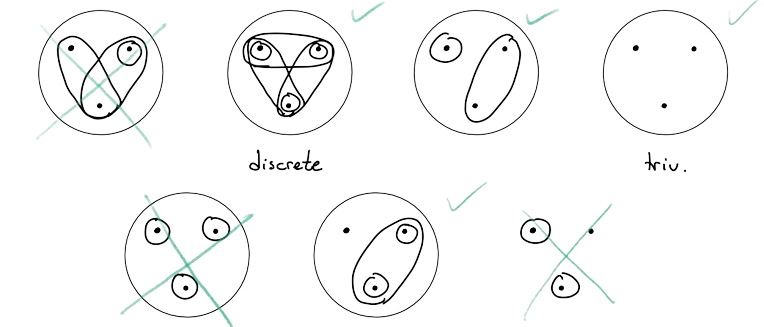
\includegraphics[scale=0.5]{diagrams/3pttop.png}
        \end{center}
        
    \end{enumerate}
    
\end{exmbox}



\begin{defbox}
    A set $\scr{B}$ of subsets of $X$ is a \emph{basis} if
    \begin{itemize}
        \item $X = \DS \bigcup_{B\in \scr{B}} B $
        \item $x\in B_1\cap B_2$ with $B_1,B_2\in \scr{B} \implies \pr{\exists B \in \scr{B}}\pr{x\in B \subseteq B_1\cap B_2 }$
    \end{itemize}
\end{defbox}

\begin{thmbox}
    A basis $\scr{B}$ generates a topology $\scr{T}$ via
    \begin{align*}
        U \in \scr{T} \iff \pr{\forall x \in U} \pr{\exists B \in \scr{B}}\pr{x \in B \subseteq U}.
    \end{align*}
\end{thmbox}
\textit{Proof.} $\emp \in \scr{T}$ (vacuously) and $X\in \scr{T}$ since $\scr{B}$ covers $X$. We then verify the union and intersection properties:
\begin{itemize}
    \item Suppose $U_\alpha \subseteq X$ are open, then $\bigcup_\alpha U_\alpha $ is open because
    \begin{align*}
        x\in \bigcup_\alpha U_\alpha \implies x \in U_\alpha \text{ for some $\alpha$} \implies x\in B_\alpha \subseteq U_\alpha \subseteq \bigcup_\alpha U_\alpha
    \end{align*}
    \item Suppose $U_1,U_2$ are open, then $U_1\cap U_2$ is open because
    \begin{align*}
        x \in U_1 \cap U_2 \implies \cases{x\in B_1\subseteq U_1\text{ for some $B_1\in\scr{B}$}\\ x\in B_2 \subseteq U_2\text{ for some $B_2\in\scr{B}$}} \implies x \in B \subseteq B_1\cap B_2 \subseteq U_1\cap U_2
    \end{align*}
    for some $B \in \scr{B}$. By induction, any finite intersection of open sets is open.\QED
\end{itemize}

\begin{exmbox}
    Let $X=\R$. We can construct three topologies via the bases:
    \begin{enumerate}
        \item $\set{(a,b): a,b\in \R}$ (the \emph{standard topology} on $\R$)
        \item $\set{[a,b): a,b\in \R}$
        \item $\set{U\subseteq \R : U = \R \setminus \set{x_1,\cdots,x_n} \text{ for some $x_1,\cdots,x_n \in \R$}}$
    \end{enumerate}
    Note, $(2)$ is finer than $(1)$, and $(1)$ is finer than $(3)$.
\end{exmbox}

\begin{whitebox}
    \textbf{Remark.} \begin{enumerate}
        \item Infinite intersections may not be open. E.g. $\bigcap_n (-1/n,1/n) = \set{0}$ is not open in the standard topology on $\R$.
        \item Different bases could generate the same topology. E.g. For $X=\R^2$, open balls generate the same topology as open squares do.
    \end{enumerate}
\end{whitebox}

\begin{defbox}
    Let $X$ be a space, and $A\subseteq X$.\begin{enumerate}
        \item $\mathrm{int}(A) = \bigcup\set{U\subseteq A: \text{$U$ is open}}$ is the \emph{interior} of $A$.
        \item $\ol{A} = \bigcap\set{C\supseteq A: \text{$C$ is closed}}$ is the \emph{closure} of $A$.
        \item $A$ is \emph{dense} if $\ol{A}=X$.
    \end{enumerate}
\end{defbox}

\begin{exmbox}
    \begin{enumerate}
        \item $\text{int}(A)=\ol{A} = A$ in the discrete topology.
        \item $\text{int}(A) = \emp; \ol{A} = X$ in the trivial topology for any $A\neq \emp,X$.
        \item $\Q$ is dense in $\R$.
    \end{enumerate}
\end{exmbox}

\begin{whitebox}
    \textbf{Warning.} $A,B$ dense does not imply $A\cap B$ dense, e.g. take $\Q$ and $\Q+\sqrt{2}$.
\end{whitebox}

\begin{thmbox}\begin{enumerate}
    \item $A \text{ open} \iff A = \text{int}(A)$
    \item $A \text{ closed} \iff A = \ol{A}$
\end{enumerate}
\end{thmbox}

\begin{defbox}
    \begin{enumerate}
        \item A \emph{neighborhood of $\pmb{x\in X}$} is an open set that contains $x$.
        \item $x\in X$ is a \emph{limit point} of $A$ if $\pr{\forall x\in U \in \scr{T}}\pr{A\cap U\setminus \set{x} \neq \emp.}$
        \item $x\in X$ is an \emph{adherent point} of $A$ if $\pr{\forall x\in U \in \scr{T}}\pr{A\cap U \neq \emp.}$
        \item The \emph{boundary} of $A$ is $\partial A = \set{x \in X : x\text{ adh pt of $A$ and $X\setminus A$}} = \ol{A} \cap \ol{X\setminus A}$.
    \end{enumerate}
\end{defbox}

\begin{thmbox}\begin{enumerate}
    \item $\ol{A} = \set{\text{adherent pts of }A} = A \cup \set{\text{limit pts of }A} = \text{int}(A) \sqcup \partial A$.
    \item $X = \text{int}(A) \sqcup \partial A \sqcup \text{int}(X\setminus A)$.
\end{enumerate}
\end{thmbox}

\begin{thmbox}
    If $U_1,U_2$ are dense and open, then $U_1\cap U_2$ is dense and open.
\end{thmbox}
\textit{Proof.} Suppose $x\in X$. We want to show that for any $x\in U $ open we have $U \cap (U_1\cap U_2) \neq \emp$. Since $U_1$ is dense, $U\cap U_1\neq \emp$. Since $U_2$ is also dense, $U\cap U_1 \cap U_2 \neq \emp$.\QED

\section{Metric Spaces}

\begin{defbox}
\begin{enumerate}
    \item A \emph{metric} on a set $X$ is a function $d:X^2\>\R$ such that
    \begin{itemize}
        \item $d(x,y)\geq 0$ and equality holds if and only if $x=y$
        \item $d(x,y) = d(y,x)$
        \item $d(x,y) + d(y,z) \geq d(x,z)$
    \end{itemize}
    The set $B_x(\eps)=\set{y: d(x,y) < \eps}$ is the (open) \emph{$\pmb{\eps}$-ball centered at $\pmb{x}$}.
    \item The \emph{metric topology} on $(X,d)$ is the topology generated by the basis
    \begin{align*}
        \scr{B} = \set{B_x (r) : x \in X, r>0}
    \end{align*}
\end{enumerate}
    
\end{defbox}


\begin{exmbox}
    The \emph{euclidean metric} $d$ on $\R^n$ is $d(\textbf{x},\textbf{y}) = \sqrt{\sum_i (x_i-y_i)^2}$.
\end{exmbox}


\section{Subspace Spaces}


\begin{defbox}
    Let $(X,\scr{T})$ be a space and $A\subseteq X$. The \emph{subspace topology} on $A$ (with respect to $X$) is
    \begin{align*}
        \scr{T}_A = \set{A\cap U : U \in \scr{T}}.
    \end{align*}
    We call $A$ with this topology a \emph{subspace} of $X$.
\end{defbox}

\begin{thmbox}
    A basis $\scr{B}$ for $\scr{T}$ defines a basis $\scr{B}_A$ for $\scr{T}_A$ via
    \begin{align*}
        \scr{B}_A = \set{A\cap B : B \in \scr{B}}.
    \end{align*}
\end{thmbox}

\begin{whitebox}
    \textbf{Remark.} If $(X,d)$ is a metric space and $A\subseteq X$ then $(A,d_A)$ is a metric space where $d_A(a_1,a_2) = d(a_1,a_2)$.
\end{whitebox}

\begin{thmbox}
    Let $(X,d)$ be a metric space. Then the metric topology on $A\subseteq X$ agrees with the subspace topology of $A\subseteq X$.
\end{thmbox}
\textit{Proof.} The subspace topology on $A$ has basis $\scr{B}_S = \set{A \cap B_x(r)}_{x\in X}$ whereas the metric topology on $A$ has basis $\scr{B}_M = \set{B^A_x(r)} = \set{A\cap B_x(r) }_{x\in A}\subseteq \scr{B}_S$. On the other hand, given any open $U$ in the subspace topology and $x\in U\subseteq A$, we have $x\in A\cap B_x(r)\subseteq U$ for some $r>0$, but this is just $x\in B^A_x(r) \subseteq U$. Since $x\in U$ was arbitrary, $U$ is open in the metric topology too.\QED

\begin{defbox}
    $A\subseteq X$ (space) is discrete if its subspace topology is discrete.
\end{defbox}

\begin{exmbox}
    Is $X = \set{0} \cup_{n} \set{1/n} $ discrete in $\R$? No. $\set{0}$ is not open in $X$. If it were, then $\exists (a,b)$ such that $(a,b)\cap X = \set{0}$, but $1/n<b$ for large $n$.
\end{exmbox}
\begin{whitebox} 
    \textbf{Warning.} $B=A=\R \times \set{0} \subseteq X=\R^2$ are examples for the following statements:\begin{enumerate}
        \item $B$ open in $A$ does not imply $B$ open in $X$.
        \item Suppose $A\subseteq Y\subseteq X$, then the $\text{int}(A)$ in $Y$ may not be $Y\cap \text{int}(A)$.  
    \end{enumerate}
\end{whitebox}
But these versions are true:
\begin{thmbox}
    \begin{enumerate}
        \item $B$ open in $A$, and $A$ open in $X$, then $B$ open in $X$.
        \item Suppose $A\subseteq Y \subseteq X$, the closure of $A$ in $Y$ is $Y\cap \pr{\text{closure of $A$ in $X$}}$.
    \end{enumerate}
\end{thmbox}

\section{Product Spaces}

\begin{defbox} Let $\set{X_\alpha}_\alpha$ be a collection of spaces. \begin{enumerate}
    \item The \emph{product topology} on $X_1\times \cdots \times X_n$ is generated by the basis $$\scr{B}=\set{Y_1\times \cdots \times Y_n: Y_1,\cdots,Y_n \text{ open}}$$
    \item More generally, the \emph{product topology} on $\prod_\alpha X_\alpha$ is generated by the basis $$\TS \scr{B}=\set{\prod_\alpha Y_\alpha: Y_\alpha \text{ open for all $\alpha$, and only finitely many $Y_\alpha\neq X_\alpha$}}$$
\end{enumerate}
\end{defbox}

\begin{thmbox}
\begin{enumerate}
    \item If $A\subseteq X; B\subseteq Y$ are subspaces, then the subspace topology and product topology on $A\times B$ agree.
    \item The metric topology on $\R^n$ agrees with the product topology on $\R^n$.
\end{enumerate}
\end{thmbox}

\section{Quotient Space}

\begin{defbox}
\begin{itemize}
    \item Let $X$ be a space, $Y$ be a set, and $q:X\>Y$ be surjective. The \emph{quotient topology} on $Y$ induced by the \emph{quotient map} $q$ is given by
    \begin{align*}
        \scr{B} = \set{U\subseteq Y: q^{-1}(U)\text{ open in }X}
    \end{align*}
    \item Let $A\subseteq X$ be a subset and define $x\stackrel{A}{\sim}y \iff x=y\text{ or }x,y\in A$. We denote $X/A$ the space on $X/\stackrel{A}{\sim}$ with quotient topology induced by the canonical map $q:X\twoheadrightarrow X/\stackrel{A}{\sim}$.
\end{itemize}
\end{defbox}

\begin{whitebox}
    \textbf{Remark.} An equivalence relation $\sim$ on $X$ determines the surjective \emph{canonical map} $q:X\twoheadrightarrow X/\sim$ defined by $q(x) = \text{equivalence class of $x$}$.
\end{whitebox}

\begin{exmbox}[bottomrule=0pt]
    \begin{enumerate}
    \item Consider the unit $2$-disk $X = D^2 = \set{x\times y : x^2+y^2 \leq 1}$. If we identify together all points on the boundary $\partial D^2$, we get the quotient space $D^2/\partial D^2$ that is homeomorphic with the subspace of $\R^3$ called the unit $2$-sphere $S^2 = \set{x\times y \times z : x^2+y^2+z^2=1}$.
    \begin{center}
    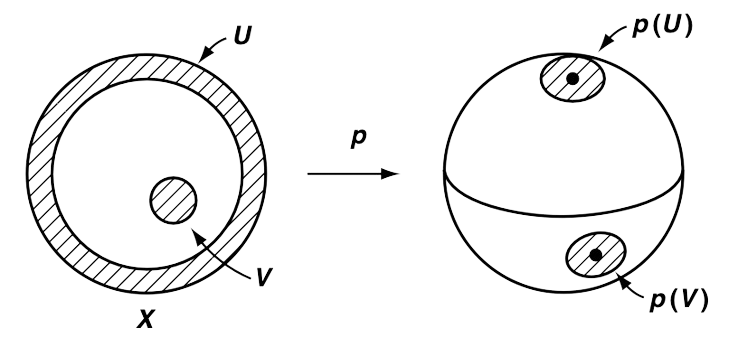
\includegraphics[scale=0.3]{diagrams/D2toS2.png}
    \end{center}
    \end{enumerate}
\end{exmbox}

\begin{redbox}[toprule=0pt]
    \begin{enumerate}
        \item[2.] We can construct a \textit{torus} $S^1\times S^1$ from the rectangle $[0,1]\times [0,1]$.
        \item[3.] We can patch two disks $D^2 \sqcup D^2$ along their boundaries to obtain $S^2$. Formally, given a homeomorphism $\phi: \partial D_1^2\> D_2^2$, we have $(D_1^2 \sqcup D_2^2)/\sim \ = S^2$ where $x\sim y \iff x=y\text{ or }x\in \partial D^2_1, y \in \partial D^2_2, \phi(x) = y$.
    \end{enumerate}
\end{redbox}

\section{Continuous Functions}

\begin{defbox}
    Let $X,Y$ be spaces. A function $f:X\>Y$ is
    \begin{itemize}
        \item \emph{continuous at $\pmb{x\in X}$} if $f^{-1}(V)$ is open in $X$ for all neighborhoods $V$ of $f(x)$.
        \item \emph{continuous} if $f^{-1}(V)$ is open in $X$ for all $V$ open in $Y$.
        \item a \emph{homeomorphism} if $f$ is bijective, and $f$ and $f^{-1}$ are continuous.
    \end{itemize}
\end{defbox}

\begin{thmbox}
    \begin{enumerate}
        \item Let $\scr{B}$ be a basis of $X$. The map $f:X\>Y$ is continuous if and only if $f^{-1}(B)$ is open for all $B\in \scr{B}$.
        \item A composition of continuous functions is continuous.
        \item Let $A\subseteq X$ be a subspace and $f:X\>Y$ be continuous. Then $f\mid_A$ is continuous.
        \item[4.] Let $f:Z\> X\times Y$ where $f = f_X\times f_Y$. Then $f$ is continuous if and only if $f_X,f_Y$ are continuous.
        \item[5.] Any quotient map is continuous. Given a quotient map $q:X\> Y$, $f:Y\> Z$ is continuous if and only if $g = f\circ q$ is continuous.\vspace{-0.2cm}
        \begin{center}
            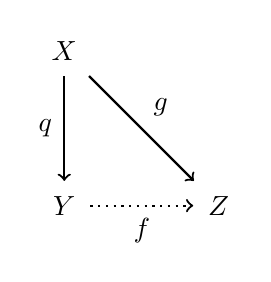
\begin{tikzpicture}[->, thick,main/.style={inner sep = 5pt, minimum size = 0.6cm},edge/.style={midway, inner sep=4pt, minimum size=0.4cm} , scale = 0.7]
    
            \node[main] (00) at (0,0) {$Y$};
            \node[main] (01) at (0,2.8) {$X$};
            \node[main] (10) at (2.8,0) {$Z$};
        
            \path
                (01) edge node[edge, above right] {$g$} (10)
                (01) edge node[edge, left] {$q$} (00)
                (00) edge[dotted] node[edge, below] {$f$} (10)
                ;
            \end{tikzpicture}
        \end{center}\vspace{-0.7cm}
        \item[6.] The following are equivalent to $f:X\>Y$ being continuous:
        \begin{itemize}
            \item[(1)] $f^{-1}(C)$ is closed for all closed $C\subseteq Y$.
            \item[(2)] Given any $x\in X$ and $f(x) \subseteq V$ open, there exists open $U$ with $f(U)\subseteq V$.
            \item[(3)] $f\pr{\ol{A}} \subseteq \ol{f(A)}$ for all $A\subseteq X$.
        \end{itemize}
    \end{enumerate}
\end{thmbox}
\textit{Proof of (6).} \begin{itemize}
    \item Continuity is equivalent to (1) by taking complements.
    \item For (2), say $f$ is continuous, then $U = f^{-1}(V)$ works. Conversely, say (2) is true. Then for any open $V\subseteq Y$, any $v\in V$ admits a neighborhood within $V$, which has an open preimage $U_v\subseteq X$. Then $f^{-1}(V) = \bigcup_{v\in V} U_v $ is open, and thus $f$ is continuous.
    \item $(1)\Rightarrow (3)$. Since $A\subseteq f^{-1}(f(A)) \subseteq f^{-1}\pr{\ol{f(A)}}$ which is closed, we have $\ol{A}\subseteq f^{-1}\pr{\ol{f(A)}}$ and thus $f\pr{\ol{A}}\subseteq \ol{f(A)}$. 
    \item $(3)\Rightarrow (1)$. Let $C\subseteq Y$ be closed. Then $f\pr{\ol{f^{-1}(C)}} = \ol{f\pr{f^{-1}(C)}}\subseteq \ol{C} = C$ and hence $\ol{f^{-1}(C)}\subseteq f^{-1}f\pr{\ol{f^{-1}(C)}}\subseteq f^{-1}(C)$ and thus $f^{-1}(C)$ is closed.\QED
\end{itemize}

\begin{corollary}
    Say $X,Y$ are metric spaces. $f:X\>Y$ is continuous if and only if
    \begin{align*}
        \pr{\forall x \in X,\eps>0}\pr{\exists\delta>0}\pr{\forall d_X(x,y)<\delta}\pr{d_Y\pr{f(x),f(y)} < \eps}.
    \end{align*}
\end{corollary}

\begin{thmbox}
    \textbf{(Pasting Lemma)} Let $X = A\cup B$ be a space where $A,B$ are closed. If $f_A:A\>Y$ and $f_B:B\>Y$ are continuous and $f_A(x) = f_B(x)$ for all $x\in A\cap B$, then $f:X\>Y$ defined by
    \begin{align*}
        f(x) = \cases{
        f_A(x) & x\in A\\
        f_B(x) & x\in B\\
        }
    \end{align*}
    is continuous.
\end{thmbox}

\section{Limits and Continuity}

\begin{defbox}
    $\set{x_n}_{n\in \N}$ in $X$ \emph{converges} to $x\in X$ if any neighborhood of $x$ contains all but finitely many $x_n$. Write $x_n\> x$.
\end{defbox}

\begin{whitebox}
    \textbf{Warning.} Limits may not be unique:
    \begin{enumerate}
        \item In the trivial topology, any sequence converges to all points.
        \item In $\R_1 \sqcup \R_2 / \sim$ where $x\sim y \iff x\in \R_1, y\in \R_2, x=y\neq 0$, we have
        \begin{align*}
            1/n \> 0_1 \quad \text{and} \quad 1/n \> 0_2 \quad \text{(\emph{fat point})}
        \end{align*}
    \end{enumerate}
\end{whitebox}

\begin{thmbox}
    If $x_n\> x$, then $x\in \ol{\set{x_n}_n}$.
\end{thmbox}

\begin{defbox}
    A space $X$ is \emph{first-countable} if for any $x\in X$, there exists a countable number of neighborhoods $U_1,U_2,\cdots$ such that any neighborhood of $x$ contains some $U_i$. The $\set{U_i}$ is called a \emph{neighborhood basis} of $x$.
\end{defbox}

\begin{thmbox}
    If $X$ is first-countable,
    \begin{enumerate}
        \item $x\in \ol{A} \implies \exists x_1,x_2,\cdots \in A$ such that $x_n\> x$.
        \item $f:X\> Y$ is continuous if and only if $\pr{x_n\>x} \implies \pr{f(x_n) \> f(x)}$.
    \end{enumerate}
\end{thmbox}

\section{Connectedness}

\begin{defbox}
    A space $X$ is \emph{connected} if there is no nontrivial clopen (closed and open) set $A\subseteq X$.
\end{defbox}

\begin{exmbox}
    The subspace $(0,1)\cup (2,3)$ of $\R$ is not connected.
\end{exmbox}

\begin{thmbox}
    $[a,b]\subseteq \R$ is connected.
\end{thmbox}
\textit{Proof.} Suppose the contrary, that $[a,b]=A\sqcup B$ where $A,B$ are closed and non-empty. WLOG Assume $b\in B$. Then $s = \sup A < b$. If $s\in A$, since $A$ is also open, there exists $(s-\eps,s+\eps) \subseteq A \implies \sup A \geq s+\eps$, a contradiction. Hence $s\in B$ instead. Since $B$ is open, there exists $(s-\eps,s+\eps) \subseteq B$ and thus $\sup A \leq s-\eps$, a contradiction.\QED

\begin{defbox}
    A space $X$ is \emph{path-connected} if every pair $x,y\in X$ can be joined by a \textit{path} in $X$: a continuous map $\gamma :I=[0,1]\>X$ such that $\gamma(0)=x$ and $\gamma(1)=y$. 
\end{defbox}

\begin{exmbox}
    \begin{enumerate}
        \item $\R^n$ is path-connected. Use the path $\gamma (t) = t \textbf{x} + (1-t) \textbf{y}$.
        \item $S^n$ is path-connected. Use the path $\gamma (t) = \dfrac{t \textbf{x} + (1-t) \textbf{y}}{\abs{t \textbf{x} + (1-t) \textbf{y}}}$.
        \item A torus is path-connected: Start with a path in $I^2$ and then take the quotient.
    \end{enumerate} 
\end{exmbox}

\begin{thmbox}
    \begin{enumerate}
        \item Any path-connected space is connected.
        \item If $f:X\>Y$ is continuous and surjective, 
        \begin{itemize}
            \item $X$ connected $\implies Y$ connected.
            \item $X$ path-connected $\implies Y$ path-connected.
        \end{itemize}
        \item Quotients of a (path-)connected space is (path-)connected.
        \item A product of (path-)connected spaces is (path-)connected.
    \end{enumerate}
\end{thmbox}

\begin{exmbox}
The \emph{topologist's sine curve} defined by $$X = \set{(x\times \sin(1/x)): x>0} \cup \set{0}\times [-1,1]$$
is connected but not path-connected.
    \begin{center}
        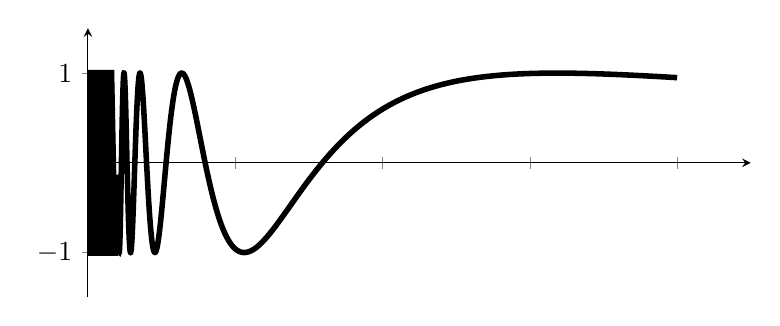
\begin{tikzpicture}
        \begin{axis}[
            domain=0.04:0.8, 
            samples=8000, %change to 8000
            axis lines=center, 
            xlabel={}, 
            ylabel={}, 
            xtick={},
            xticklabels={},
            ytick={},
            xmin=0, xmax = 0.9,
            ymin=-1.5, ymax=1.5,
            width=10cm, height=5cm
        ]
            \addplot[line width = 2pt] {sin(deg(1/x))};
            \draw[fill=black] (axis cs:0,-1.03) -- (axis cs:0.04,-1.03) -- (axis cs:0.035,1.03) -- (axis cs:0,1.03);
        \end{axis}
    \end{tikzpicture}
    \end{center}
\end{exmbox}

\begin{defbox}
    The equivalence relation $x\sim y$ where there is a (path-)connected subspace containing both $x,y$ partitions the space into (path-)connected \emph{components}.
\end{defbox}

\section{Compactness}

\begin{defbox}
    \begin{enumerate}
        \item An \emph{open cover} of $X$ is a collection of open sets that cover $X$. A space $X$ is \emph{compact} if every open cover of $X$ admits a finite subcover.
        \item A space $X$ is \emph{sequentially compact} if every sequence of points in $X$ admits a convergent subsequence.
    \end{enumerate}
    
\end{defbox}

\begin{thmbox}
    1st-countable $+$ compact $\implies$ sequentially compact.
\end{thmbox}
\textit{Proof.} Suppose $\set{x_n}_n$ does not have a convergent subsequence. Let $x\in X$, then there exists a countable neighborhood basis $U_1,U_2,\cdots$. We can safely let $U_1\supseteq U_2 \supseteq \cdots$ by taking successive intersections. Since there is no subsequence that converges to $x$, only finitely many $x_n$ lie in $U_n$ for some sufficiently large $n$. Hence, every $x\in X$ has a neighborhood $U_x$ that intersects $\set{x_n}_n$ at a finite number of points. Taking the union of all $U_x$ and applying compactness shows that $\set{x_n}_n$ is finite, so we can conclude by the pigeonhole principle.\QED

\begin{thmbox}
    \begin{enumerate}
        \item Every closed subspace of a compact space is compact.
        \item A continuous function maps compact spaces to a compact image.
        \item Suppose $X$ is compact and $C_1\supseteq C_2\supseteq \cdots$ is a sequence of closed and non-empty sets. Then $\bigcup_n C_n$ is non-empty.
        \item A product of compact spaces is compact (Infinite case is hard: Tychonoff's Thm)
        \item $[a,b]$ is compact.
    \end{enumerate}
\end{thmbox}
\textit{Proof of (4).} Suppose $[a,b]=\bigcup_\alpha U_\alpha$. Then $$S=\set{x\in[a,b]: [a,b] \text{ can be covered by finitely many $U_\alpha$}}$$ contains $a\in S$ and is bounded above by $b$. Hence $S$ has a supremum $s$. 
\begin{whitebox}
    \textbf{Claim.} $s\in S$.\\
    \textit{Proof.} Let $s\in U_\beta$ for some $\beta$, so there exists $(s-\eps,s+\eps)\subseteq U_\beta$. If $s\not\in S$, just add $U_\beta$ to the finite subcover of $[a,s-\eps/2]$.\qed \vspace{0.4cm}\\
    \textbf{Claim.} $s=b$.\\
    \textit{Proof.} If not, then similarly, just add $U_\beta$ to the finite subcover of $[a,s]$.\qed
\end{whitebox}
Therefore $[a,b]$ can be covered by finitely many $U_\alpha$.\QED
\begin{thmbox}
    \textbf{(Heine-Borel)}\\ A subspace $A$ of $\R^n$ is compact if and only if it is closed and bounded.
\end{thmbox}
\textit{Proof.}
\begin{itemize}
    \item $(\Leftarrow)$ $X\subseteq [-M,M]^n$ is a closed subset of a compact space, so $X$ is compact.
    \item $(\Rightarrow)$ Compactness on the open cover $\set{B_0(r)}_{r>0}$ shows $X$ is bounded. We then show any limit pt $x$ of $X$ is in $X$: For all $n\in\N^*$, $C_n:=\ol{B_x{1/n}}\cap X \neq \emp$, and thus $ \bigcap_n C_n = X\cap\set{x}$ is non-empty.\QED
\end{itemize}

\section{Hausdorff Spaces}

\begin{defbox}
    A space $X$ is \emph{Hausdorff} if for any distinct $x,y\in X$ there exists disjoint neighborhoods $x\in U, y\in V$.
\end{defbox}

\begin{exmbox}
    \begin{enumerate}
        \item The trivial topology is not Hausdorff. The discrete topology is.
        \item Metric spaces are Hausdorff.
        \item The finite complement topology on $\R$ is not Hausdorff.
        \item The space $\R_1\sqcup \R_2/\sim$ containing the fat point is not Hausdorff.
    \end{enumerate}
\end{exmbox}

\begin{thmbox}
    $X$ is Hausdorff if and only if $\Delta = \set{(x\times x): x\in X}\subseteq X^2$ is closed.
\end{thmbox}
\textit{Proof.}
\begin{itemize}
    \item $(\Rightarrow)$ If $X$ is Hausdorff, for any $x\neq y$ there exists disjoint neighborhoods $U,V$ of $x,y$ respectively. Then $U\times V$ is a neighborhood of $(x\times y)\in X\times Y$ disjoint from $\Delta$. Taking the union over all $(x\times y)$ implies $\Delta$ is closed.
    \item $(\Leftarrow)$ If $\Delta$ is closed, given any $x\neq y$ there exists a basis neighborhood $U\times V$ of $(x\times y)$ disjoint from $\Delta$. Then $U,V$ are the desired neighborhoods.\QED
\end{itemize}

\begin{thmbox}
    \begin{enumerate}
        \item In a Hausdorff space, a sequence of points converge to at most one point.
        \item One-point sets in a Hausdorff space are closed.
        \item A subspace of a Hausdorff space is Hausdorff.
        \item A finite product of Hausdorff spaces is Hausdorff.
        \item A compact subspace of a Hausdorff space is closed.
    \end{enumerate}
\end{thmbox}
\begin{whitebox}
    \textbf{Warning.} A quotient of a Hausdorff space may not be Hausdorff.
\end{whitebox}

\section{Normal Spaces} \label{normchapter}

\begin{defbox}
\begin{enumerate}
    \item $X$ is $\pmb{T_1}$ if one-point sets are closed.
    \item A space is \emph{normal} if it is $T_1$, and, for any pair of disjoint closed sets $A,B\subseteq X$ there exists disjoint open sets $U,V\subseteq X$ such that $A\subseteq U, B\subseteq V$.
\end{enumerate}
\end{defbox}

\begin{whitebox}
    \textbf{Remark.} \begin{enumerate}
        \item Normal $\implies$ Hausdorff $\implies T_1$.
        \item A quotient, subspace, or product of normal space(s) need not be normal.
    \end{enumerate}
\end{whitebox}

\begin{exmbox}
    \begin{enumerate}
        \item The fat point $\R_1\sqcup \R_2/\sim$ is $T_1$ but not Hausdorff.
        \item The \emph{$\pmb{K}$-topology} on $\R$ generated by $\set{(a,b)}\cup\set{(a,b)\setminus \bigcup_n\set{1/n}}$ is Hausdorff but not normal.
        \item The topology $\R_\ell$ on $\R$ generated by $\set{[a,b)}$ is normal, but $\R_\ell^2$ is not normal.
    \end{enumerate}
\end{exmbox}

\begin{thmbox}
    \begin{enumerate}
        \item A closed subspace $A$ of a normal space $X$ is normal.
        \item Compact $+$ Hausdorff $\implies$ Normal.
    \end{enumerate}
\end{thmbox}
\textit{Proof of (2).} Suppose $A,B\subseteq X$ are disjoint and closed. Fix $a\in A$. Then for each $b\in B$ there exists disjoint neighborhoods $a\in U_{b}, b\in V_{b}$. Since $B$ is also compact, there exists finitely many $V_{b}$ that cover $B$. The union of such finitely many $V_{b}$ and the intersection of their corresponding $U_{b}$ form disjoint open sets containing $a$ and $B$ respectively. Repeat the same procedure for every $a\in A$ and then apply compactness of $A$. \QED

\begin{thmbox}
    Metric spaces are normal.
\end{thmbox}
\textit{Proof.} We can show that, for any subset $A\subseteq X$, the \textit{point-to-set distance} $d(-,A):X\>\R$ given by $d(x,A) = \under{inf}{a\in A}\ d(x,a)$ is continuous. For disjoint closed sets $A,B$, the open sets
\begin{align*}
    U = \set{x : d(x,A) < d(x,B)}, \qquad V = \set{x : d(x,A) > d(x,B)}
\end{align*}
contain $A,B$ respectively and are disjoint.\QED

\begin{thmbox}
    $X$ is normal if and only if for any closed $A$ and open $U$ such that $A\subseteq U$, there exists an open set $V$ such that $A \subseteq V \subseteq \ol{V} \subseteq U$.
    \label{regnormlocal}
\end{thmbox}

\begin{thmbox}
    \textbf{(Urysohn's Lemma)}\\
    Let $X$ be normal and $A,B$ be disjoint closed sets of $X$. There exists a continuous map
    \begin{align*}
        f: X \> I
    \end{align*}
    such that $f(A) = \set{0}$ and $f(B)=\set{1}$.
\end{thmbox}
\textit{Proof.} Define open sets $U_p$ for each $p\in\Q \cap [0,1]$ as follows: Enumerate $\Q \cap [0,1]$ such that 1 and 0 are the first two elements. Define $U_1=X-B$ and by normality pick $U_0$ such that $A \subseteq U_0\subseteq \ol{U_0} \subseteq U_1$. By induction, say we defined $U_p$ for a finite number of $p$'s and let $r$ be the next rational in the enumeration. We must have $p<r<q$ where $U_p,U_q$ are already defined. By normality we pick $U_r$ such that $\ol{U_p}\subseteq U_r \subseteq \ol{U_r}\subseteq U_q$. 
\x
Additionally, we let $U_p = \emp$ for all rationals $p<0$ and $U_p = X$ for all rationals $p>1$. Hence, 
\begin{align*}
    p < q \imply \ol{U_p}\subseteq U_{q}.
\end{align*}
We then define $f(x) =\DS \inf\set{ p: x\in U_p}$. It is easy to see $f(A) = \set{0}$ and $f(B)=\set{1}$. We show that $f$ is continuous.
\begin{whitebox}
    \textbf{Lemma 1.} $x\in \ol{U_r} \imply f(x) \leq r$\\
    \textit{Proof.} If $x\in \ol{U_r}$, then $x\in U_s$ for every $s>r$. Hence $f(x) \leq r$.\qed
    \vspace{5pt}\\
    \textbf{Lemma 2.} $x\not\in \ol{U_r} \imply f(x) \geq r$.\\
    \textit{Proof.} If $x\not\in \ol{U_r}$, then $x\not\in U_s$ for any $s<r$. Hence $f(x) \geq r$.\qed
\end{whitebox}
Given a ball $I = (f(x)-\delta,f(x)+\delta)$, we wish to find a neighborhood $U$ of $x$ such that $f(U)\subseteq I$. First we choose rational numbers $p,q\in I$ such that $p<f(x) < q$. Then the open set $U_q \setminus \ol{U_p}$ is the desired neighborhood using the lemmas above.\QED

\begin{thmbox}
    \textbf{(Tietze Extension Theorem)}\\
    Let $A$ be closed in a normal space $X$. Any continuous map from $A$ to $I$ can be extended to a continuous map from $X$ to $I$. True also for $\R$ instead of $I$.
\end{thmbox}
\newpage
\textit{Proof.} We show for $[-1,1]$ instead of $I$, and then for $(-1,1)$ instead of $\R$.
\begin{whitebox}
    \textbf{Lemma.} If $f:A\>[-\eps,\eps]$ is continuous, there exists continuous $g:X\>\R$ with
    $g(X) \subseteq [-\eps/3,\eps/3]$ and $(g-f)(A) \subseteq [-2\eps/3,2\eps/3]$.\vspace{5pt}\\
    \textit{Proof.} Applying the Urysohn Lemma on the disjoint closed sets $L=f^{-1}([-\eps,-\eps/3])$ and $R=f^{-1}([\eps/3,\eps])$, there exists $g:X\>[-\eps/3,\eps/3]$ such that $g(L)= \set{-\eps/3}$ and $g(R) = \set{\eps/3}$. This $g$ works.\qed
\end{whitebox}
Now let $f:A\> [-1,1] $ be continuous. Then we can find $g_1:X\>[-1/3,1/3]$ such that $|f(a) - g_1(a)|\leq 2/3$ for all $a\in A$. Then we apply the Lemma on $f-g_1$ again, so we get $g_2: X\> [-2/9,2/9]$ such that $|f(a)-g_1(a)-g_2(a)|\leq 4/9$. Recursively, we get a sequence of functions $g_n$ such that $g_{n+1}:X\> [-(2/3)^n/3, (2/3)^n/3]$ and 
\begin{align*}
    |f(a) - g_1(a) - \cdots - g_{n+1}(a)|\leq\pr{\frac23}^{n+1}.
\end{align*}
By the Weierstrass $M$-test, $\DS g(x) = \sum_{n=1}^\infty g_n(x)$ converges to the desired function (Exercise). 
\x
To show the $(-1,1)$ version, take $g$ from the $[-1,1]$ case. Apply the Urysohn Lemma to the disjoint closed sets $A$ and $D=g^{-1}(\set{-1})\cup g^{-1}(\set{1})$ to get a continuous $\phi:X\>[0,1]$ so that $\phi(D)=\set{0}$ and $\phi(A)=\set{1}$. Then $h(x) = \phi(x) g(x) $ works ($\abs{h(x)}<1$).\QED


\chapterpart{Urysohn Metrization Theorem}

\begin{defbox}
    \begin{enumerate}
        \item A space is \emph{second-countable} if it has a countable basis.
        \item A space is \emph{metrizable} if it is homeomorphic to a metric space.
    \end{enumerate}
    
\end{defbox}

\begin{thmbox}
    \textbf{(Urysohn Metrization Theorem)}\\
    2nd countable $+$ Normal $\implies$ Metrizable.
\end{thmbox}
\textit{Proof.} We first note that $I^\omega = \set{\textbf{x}= (x_1,x_2,\cdots) : x_i \in I}$ with the metric
\begin{align*}
    d(\textbf{x},\textbf{y}) = \sup_n \frac{\abs{x_n-y_n}}{n}.
\end{align*}
is a metric space. Let $X$ be normal with a countable basis $\scr{B}$. We will embed $X$ into $I^\omega$. 
\begin{whitebox}
    \textbf{Lemma.} There exists a collection $\set{f_n: X\> I}_{n\in\N}$ of continuous functions such that given any $x\in X$ and any neighborhood $U$, there exists some $f_n$ that is positive at $x$ but vanishes outside $U$.\vspace{5pt}\\
    \textit{Proof.} For each $B,C\in \scr{B}$ with $\ol{B}\subseteq C$, apply the Urysohn Lemma to construct a continuous function $g_{B,C}:X\>I$ such that $g_{B,C}\pr{\ol{B}} = \set{1}$ and $g_{B,C}(X\setminus C) = \set{0}$. $\set{g_{B,C}: \ol{B}\subseteq C}$ is the desired collection. It is countable because $\scr{B}\times \scr{B}$ is countable, and given any $x$ with neighborhood $U$, we can choose by Theorem \ref{normchapter}.\ref{regnormlocal} the sequence of open sets $x\in B \subseteq \ol{B} \subseteq C \subseteq U$, and then use $g_{B,C}$.\qed
\end{whitebox}
Using $\set{f_n}_{n\in\N}$ from the Lemma, define $F:X\> I^\omega$ such that
\begin{align*}
    F(x) = \pr{f_0(x), f_1(x), f_2(x), \cdots}
\end{align*}
\begin{itemize}
    \item $F$ is injective because given $x\neq y$, there exists some $f_n(x)>0=f_n(y)$ (Hausdorff!).
    \item $F$ is continuous: Let $B_x(\eps)\subseteq I^\omega$. Fix an integer $N > 2/\eps$. Since each $f_n$ is continuous, for each $1\leq n \leq N$ there exists a neighborhood $x\in U_n$ such that $y\in U_n \implies \abs{f_n(x)-f_n(y)}\leq \eps/2$. Hence for any $y\in U_1\cap\cdots\cap U_N$,
    \begin{align*}
        d\pr{F(x),F(y)} &= \sup_n \frac{\abs{f_n(x)-f_n(y)}}{n}\\
        &\leq \max\pr{\sup_{1\leq n\leq N} \frac{\abs{f_n(x)-f_n(y)}}{n},\sup_{n> N} \frac{\abs{f_n(x)-f_n(y)}}{n} }\\
        &\leq \max \pr{\frac{\eps}{2}, \frac{1}{N+1}} < \eps.
    \end{align*}
    \item For each open set $U$ in $X$, $F(U)$ is open in $F(X)$: Let $x\in U$ and $f(x) = z$. Choose a $f_N$ that is positive at $x$ but vanishes outside $U$. Let
    \begin{align*}
        W = F(X) \cap \pi_N^{-1}\pr{(0,1]}
    \end{align*}
    be open in $F(X)$. We claim that $z\in W \subseteq F(U)$. Firstly, we have $z=F(x)\in W$ because $f_N(x)>0$. Secondly, given any $F(y) \in W$, we must have $f_N(y)>0$. Since $f_N$ vanishes outside $U$, $y$ must be in $U$, so $F(y) \in F(U)$.
\end{itemize}
Therefore, $X$ is homeomorphic to its image under $F$, a subspace of the metric space $I^\omega$, which is also a metric space.\QED


\section{Manifolds}\label{manifoldsec}

\begin{defbox}
    An \emph{$\pmb{n}$-manifold} is a 2nd countable Hausdorff space $X$ such that each $x\in X$ has a neighborhood homeomorphic with an open subset of $\R^n$. We also write $X=X^n$. A 1-manifold is a \emph{curve}, and a 2-manifold is a \emph{surface}.
\end{defbox}

\begin{thmbox}
    $X^n\times Y^m$ is an $(n+m)$-manifold.
\end{thmbox}
\textit{Proof.} Hausdorffness and 2nd Countability follow immediately. Fix $(x\times y )\in X\times Y$, then there exists neighborhoods $U,V$ of $x,y$ homeomorphic to $\R^n,\R^m$ respectively. Then $U\times V$ is a neighborhood of $(x\times y)$ homeomorphic to $\R^n\times\R^m \cong \R^{n+m}$.\QED

\begin{exmbox}
    \begin{enumerate}
        \item $\R^n$ is an $n$-manifold.
        \item $S^n$ is an $n$-manifold. (Write $S^n = e_1^n \cup e_2^n$ where $e^n = \text{int}\pr{D^n}\cong \R^n$).
        \item The \emph{real projective space} $\R \mathbb{P}^n = S^n/\sim$ (where $x\sim y \iff x=\pm y$) is an $n$-manifold.
        \item $T^n = \underbrace{S^1\times \cdots S^1}_{n}$ is an $n$-manifold. $T^2$ is a \emph{torus}.
        \item \textit{Fact:} Every connected curve is homeomorphic to either $\R$ and $S^1$.
    \end{enumerate}
\end{exmbox}

\begin{thmbox}
    A compact $n$-manifold $X$ can be embedded in $\R^N$ for some $N\in\N$.
\end{thmbox}
\textit{Proof.} Each $x\in X$ admits a neighborhood $U^x$ with a homeo $\phi^x: \R^n \> U^x$. We can choose a basis $x\in B^x \subseteq \phi^x\pr{B_0(1)}$, and hence by compactness of $X$ via the $B^x$ there exists $U_1,\cdots,U_m$ with homeos $\phi_i: \R^n\> U_i$ and $X \subseteq \bigcup_i \phi_i\pr{B_0(1)}$ 
\x
By Urysohn's Lemma, there exists $\rho_i: X \> I$ such that $\rho_i\pr{\ol{\phi_i\pr{B_0(1)}}} = \set{1}$ and $\rho_i\pr{X\setminus \phi_i\pr{B_0(2)}} = \set{0}$. Via the pasting lemma, let $\psi_i: X\> 
\R^{n}$ be the continuous function
\begin{align*}
    \psi_i(x) = \cases{\rho_i(x)\phi^{-1}_i(x) & \text{$x\in U_i$}\\ (0,\cdots,0) &\text{otherwise}}.
\end{align*}
\begin{center}
    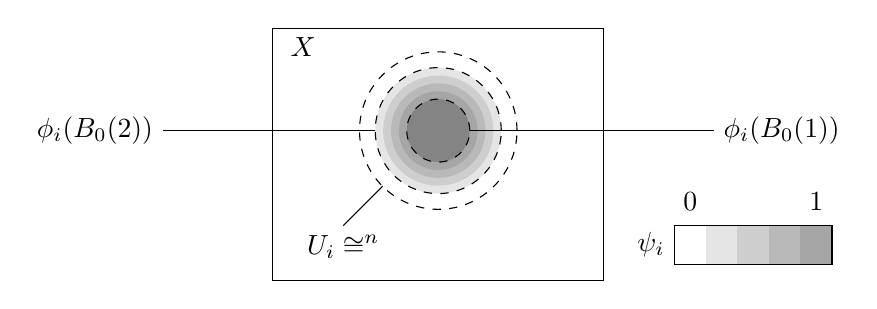
\begin{tikzpicture}
        \fill[opacity= 0.2] (0,0) circle (0.4);
        \draw[dashed] (0,0) circle (0.4);
        
        \fill[opacity= 0.1] (0,0) circle (0.5);
        \fill[opacity= 0.1] (0,0) circle (0.6);
        \fill[opacity= 0.1] (0,0) circle (0.7);
        
        \fill[opacity= 0.1] (0,0) circle (0.8);
        \draw[dashed] (0,0) circle (0.8);
        \draw[dashed] (0,0) circle (1);
        \draw (0.4,0) -- ++(3.1,0) node[right] {$\phi_i(B_0(1))$};
        \draw (-0.8,0) -- ++(-2.7,0) node[left] {$\phi_i(B_0(2))$};
        \draw (-0.707, -0.707) -- ++(-0.5,-0.5) node[below] {$U_i\cong \R^n$};
        \draw (-2.1,-1.9) rectangle (2.1,1.3);
        \draw (-2,1.3) node[below right] {$X$};
        \draw (3, -1.7) rectangle ++(2,0.5); 
        \draw (3, -1.45) node[left] {$\psi_i$};
        \fill[opacity=0.1] (5, -1.2) rectangle ++(-0.4,-0.5);
        \fill[opacity=0.1] (5, -1.2) rectangle ++(-0.8,-0.5);
        \fill[opacity=0.1] (5, -1.2) rectangle ++(-1.2,-0.5);
        \fill[opacity=0.1] (5, -1.2) rectangle ++(-1.6,-0.5);
        \draw (3.2, -0.9) node {0};
        \draw (4.8, -0.9) node {1};
    \end{tikzpicture}
\end{center}
Then $F(x) = (\rho_1(x),\cdots,\rho_m(x),\psi_1(x),\cdots,\psi_m(x))$ embeds $X$ into $\R^{m(n+1)}$.\QED

\section{Paracompactness}\label{parachap}

\begin{defbox}
    \begin{itemize}
        \item An open cover $\set{U_\alpha}_\alpha$ of $X$ is \emph{locally finite} if every $x\in X$ has a neighborhood that intersects only finitely many $U_\alpha$.
        \item A \emph{refinement} of an open cover $\set{U_\alpha}_\alpha$ of $X$ is an open cover $\set{V_\beta}_\beta$ such that each $V_\beta$ is contained in some $U_\alpha$ (depends on $\beta$).
        \item A space $X$ is \emph{paracompact} if it is Hausdorff, and, every open cover of $X$ admits a locally finite refinement.
    \end{itemize}
    
\end{defbox}

\begin{whitebox}
    \textbf{Warning.} \begin{enumerate}
        \item Some sources do not require Hausdorffness in the definition.
        \item Quotient/Subspace/Product of paracompact space(s) may not be paracompact.
    \end{enumerate}
\end{whitebox}

\begin{exmbox}\label{Rnparac}
    $\R^n$ is paracompact. Let $B(r)$ be the open ball of radius $r$ centered at the origin. Given any open covering $\scr{A}$, for each $n\in\N^*$ we can pick a finite number of elements of $\scr{A}$ that covers $\ol{B(n)}$. Intersect them with $\R^n \setminus \ol{B(n-1)}$. The union of these open sets is a desired locally finite refinement.
\end{exmbox}

\begin{thmbox}
    \begin{enumerate}
        \item A closed subspace of a paracompact space is paracompact.
        \item Compact $+$ Hausdorff $\implies$ Paracompact
        \item Metric space $\implies$ Paracompact.
        \item Paracompact $\implies$ Normal.
    \end{enumerate}
\end{thmbox}
\textit{Proof of (4).} Let $A,B$ be closed and disjoint. We first prove the case when $A=\set{a}$. For each $b\in B$ pick disjoint neighborhoods $a\in U_b, v\in V_b$. Since $(X\setminus B) \cup_b V_b$ is an open cover of $X$, by paracompactness there exists a locally finite refinement of $V_\alpha$'s that cover $B$. Also, $x$ has a neighborhood $W$ that intersects only finitely many $V_\alpha$, say $V_{b_1},\cdots,V_{b_n}$. Then the open sets $U=U_{b_1}\cap\cdots\cap U_{b_n}$ and $V=V_{b_1}\cap\cdots\cap V_{b_n}$ form a desired pair.
\x
For the general case, we update the notation so that for each $a\in A$ there exists disjoint open sets $a\in U_a, B\subseteq V_a$. Let $\set{U_\alpha}$ be a locally finite refinement that covers $A$, so $b\in B$ admits a neighborhood $W_b$ that intersects finitely many $U_\alpha$, say $U_{a_1},\cdots,U_{a_n}$. We then let $V_b = W_b \cap_i V_{a_i}$. Then $U=\bigcup_\alpha U_\alpha$ and $V=\bigcup_{b\in B} V_b$ give the desired separation.\QED

\begin{defbox}
    A \emph{partition of unity} on $X$ for a locally finite open cover $\set{U_\alpha}_{\alpha}$ is a collection of continuous $\rho_\alpha: X\> I$ such that\begin{itemize}
        \item $\rho_\alpha(x)>0\implies x\in U_\alpha$
        \item $\sum_\alpha \rho_\alpha(x)=1$ (well-defined due to local finiteness)
    \end{itemize}\label{partunityfinite}
\end{defbox}

\begin{thmbox}
    Every cover of a paracompact space admits a refinement that has a partition of unity.
\end{thmbox}
\textit{Proof.} Let $\set{U_\alpha}$ be a cover of $X$. For each $x\in X$ there is an $x\in U_{\alpha_x}$ and hence we can pick $x\in W_x \subseteq \ol{W_x}\subseteq U_{\alpha_x}$ by normality. Let $\set{V_\beta}$ be a locally finite refinement of $\set{W_x}$. By Urysohn's Lemma, there exists $\psi_\beta:X\>I$ such that $\psi\pr{\ol{V_\beta}}=\set{1}$ and $\psi\pr{X\setminus U_{\alpha_\beta}}=\set{0}$. Then $\rho_\beta(x) = \psi_\beta(x)/\sum_\gamma \psi_\gamma(x)$ is a desired partition of unity.\QED

\begin{thmbox}\label{maniparac}
    Manifold $\implies$ Paracompact.
\end{thmbox}
\textit{Proof.} We first prove that a manifold $X$ can be a limit of increasing compact sets.

\begin{whitebox}
    \textbf{Lemma.} $\exists K_1,K_2,\cdots$ compact with $K_n \subseteq \text{int}\pr{K_{n+1}}$ and $X=\bigcup_n \text{int}(K_n)$.\\
    \textit{Proof.} Let $U_i$ with homeos $\phi_i: \R^n\> U_i$ such that $\set{\phi_i(B_0(1))}$ covers $X$. Then take the compact spaces $K_n = \bigcup_{i=1}^n \bigcup_{j=1}^n \phi_i\pr{\ol{B_0(j)}}$ for $n\in\N^*$.\qed
\end{whitebox}

Let $X=\bigcup_\alpha U_\alpha$. Then for each $n$ there exists $U^n_{1},\cdots,U^n_{t_n}$ that cover the compact space $K_n$. Then $V^n_j = U^n_j\setminus K_{n-1}$ form a locally finite refinement: Any $x\in X$ is contained within some $\text{int}(K_n)$, which means it can only be in the sets $V^m_j$ $(1\leq j \leq t_m)( 1\leq m \leq n)$. This is similar to Example \ref{parachap}.\ref{Rnparac}. \QED

\section{Covering Dimension}

\begin{defbox}
    \begin{enumerate}
        \item The \emph{covering dimension} of a space $X$ is the infimum over $n\in\N$ such that
        \begin{align*}
            \pr{\forall \text{ open cover } \set{U_\alpha}}\pr{\exists\text{ refinement }\set{V_\beta}}\pr{\forall x\in X}\pr{x\text{ is in $\leq n+1$ of the }V_\beta}
        \end{align*}
        or equivalently
        \begin{align*}
            \dim X = \max_{\scr{A}\text{ open cover }X}\br{\min_{\scr{B} \text{ refmt of }\scr{A}}\underbrace{\pr{\max_{x\in X} \abs{\set{B\in \scr{B}: x\in B}}}}_{\text{\emph{order} of $\scr{B}$}}} - 1
        \end{align*}
        \item A \emph{Lebesgue number} for an open cover $\set{U_\alpha}$ of a compact metric space is a real $\delta>0$ such that any subset of $X$ of diameter $<\delta$ is contained within some $U_\alpha$.
    \end{enumerate}
\end{defbox}

\begin{thmbox}
    \textbf{(Lebesgue's Covering Lemma)}\\
    Any open cover $\set{U_\alpha}$ of a compact metric space $(X,d)$ has a Lebesgue number. 
\end{thmbox}
\textit{Proof.} Since $X$ is compact, assume $\set{U_\alpha}=\set{U_1,\cdots,U_n}$. The map $f(x) = \DS\max_{1\leq i \leq n} d(x,X\setminus U_i) > 0$ is continuous on a compact space and thus $f(X)$ has a minimum $\delta>0$.\QED


\begin{exmbox}[bottomrule=0pt]
    \begin{enumerate}
        \item Any compact subspace of $\R$ has dimension at most 1.\vspace{5pt}\\
        \textit{Proof.} Note that $\scr{C} = \set{(n,n+1),\pr{n-\frac12,n+\frac12}: n \in \Z}$ has order 2. Let $\scr{A}$ be any open covering of a compact subspace $X$ of $\R$, with some Lebesgue number $\delta>0$. The image $\scr{I}$ of $\scr{C}$ under $f:x\mapsto \delta x/2$ is an open covering whose elements have diameter $\delta/2<\delta$, and hence is an open refinement subcover of $\scr{A}$. Hence
        \begin{align*}
            \dim X &= \max_{\scr{A}\text{ open cover }X}\br{\min_{\substack{\scr{B}\text{ open refinement} \\\text{ subcover of }\scr{A}}}\pr{\text{order of }\scr{B}}} - 1\\
            &\leq \max_{\scr{A}\text{ open cover }X}\br{2} - 1 = 1.
        \end{align*}
    \end{enumerate}
\end{exmbox}
\begin{redbox}[toprule=0pt]
    \begin{enumerate}
        \item[2.] $\dim I = 1$.\vspace{5pt}\\
        \textit{Proof.} We show that there is some open covering $\scr{A}$ such that any open refinement subcover of $\scr{A}$ has order at least 2. Let $\scr{A} = \set{[0,1), (0,1]}$ and let $\scr{B}$ be any open refinement subcovering. Since $0$ and $1$ cannot belong to the same refinement, $\scr{B}$ has at least two elements. Partition $\scr{B}$ into two nonempty parts $\scr{B}_1$ and $\scr{B}_2$. If $\scr{B}$ had order 1 then $\bigcup \scr{B}_1$ and $\bigcup \scr{B}_2$ disconnect $[0,1]$, a contradiction. 
        \item[3.] \textit{Fact:} $\dim I^n = n$, and every compact subspace of $\R^n$ has dimension $\leq n$.
    \end{enumerate}
\end{redbox}

\begin{thmbox}
    \begin{itemize}
        \item If $Y$ is a closed subspace of a finite dimensional space $X$, then $\dim Y \leq \dim X$.
        \item If $X=Y\cup Z$ where $Y,Z$ are closed finite dimensional subspaces of $X$, then $\dim X = \max(\dim Y, \dim Z)$.
        \item Every compact subspace of $\R^N$ has dimension at most $N$.
    \end{itemize}
\end{thmbox}

\chapterpart{Tangent: Baire's Theorem, Function Spaces and Geometry}

\begin{defbox}
    Let $X$ be a compact metric space.
    \begin{enumerate}
        \item $\mathcal{C}\pr{X,\R^n}=\set{f:X\>\R^n \text{ cts}}$ is the metric space equipped with the uniform metric $\DS d(f,g)=\sup_x\abs{f(x)-g(x)}$.
        \item For $A\subseteq X$, $\text{diam}(A) = \DS\sup_{x,y\in A} d(x,y)$.
        \item $\Delta(f) = \sup\set{\text{diam}(f^{-1}\set{z}): z\in f(X)}$ (Deviation of $f$ from injectivity).
    \end{enumerate}
\end{defbox}

\begin{whitebox}
    \textbf{Remark.} $\DS\bigcap_n U_{1/n} = \set{f: \Delta(f)=0} = \set{f\text{ injective}}$.
\end{whitebox}

\begin{thmbox}
    \textbf{(Baire's Theorem)}\\
    Let $\set{U_n}$ be a countable collection of dense open sets in a compact Hausdorff space $X$. Then $\bigcap_n U_n$ is dense in $X$.
\end{thmbox}
\textit{Proof.} Let $W_1$ be an open set. We want to show $W_1\cap_n U_n\neq \emp$.
\begin{itemize}
    \item Since $U_1$ is dense and open, there exists $x_1\in W_1\cap U_1$ open. 
    \item Inductively, since $X$ is normal, there exists $x_n \in W_n \subseteq \ol{W_n} \subseteq W_{n-1}\cap U_{n-1}$.
\end{itemize}
Since $X$ is compact and $\ol{W_1}\supseteq \ol{W_2}\supseteq \cdots$, we have
\begin{align*}
    \emp \neq \bigcap_n \ol{W_n} \subseteq \bigcap_n \pr{U_n \cap W_n} \subseteq W \cap_n U_n.\tag*{\QED}
\end{align*}

\begin{defbox}
\begin{enumerate}
    \item $\set{z_0,\cdots ,z_m}\subseteq \R^n$ are \emph{geometrically independent} if
    \begin{align*}
        \lambda_0 z_0 + \cdots + \lambda_m z_m = \mathbf{0}, \ \lambda_0 + \cdots + \lambda_m = 0 \implies \lambda_0=\cdots=\lambda_m = 0
    \end{align*}
    \item $A\subseteq \R^n$ is in \emph{general position} if any subset of size $n+1$ are geom. ind.
\end{enumerate}
\end{defbox}

\begin{thmbox}
    Given $\set{z_0,\cdots ,z_m}\subseteq \R^n$ and $\delta>0$, there exists $\set{y_0,\cdots ,y_m}\subseteq \R^n$ that is in general position such that all $\abs{z_i-y_i}<\delta$.
\end{thmbox}

\chapterpart{Back to dimension theory}

\begin{thmbox}
    \textbf{(Embedding Compact Metric Spaces)}\\
    Every compact metric space $X$ of dimension $n$ can be embedded in $\R^{2n+1}$.
\end{thmbox}

Define $U_\eps = \set{f\in \mathcal{C}\pr{X,\R^{2n+1}} : \Delta(f)<\eps}$.

\begin{whitebox}
    \textbf{Claim.} $U_\eps$ is open. \vspace{0.5cm}\\
    \textit{Proof.} Let $f\in U_\eps$, we want to show $\exists B_f(\delta)\subseteq U_\eps$. Pick $\eps < b < \Delta(f)$ and define
    \begin{align*}
        A = \set{(x\times y): d(x,y) \geq b} \subseteq X^2
    \end{align*}
    Note that $f(x)=f(y) \implies d(x,y) \leq \Delta(f) < b \implies (x\times y)\not\in A$. Hence $\abs{f(x)-f(y)}$ has a positive minimum $2\delta$ on $A$. Now if $g\in B_f(\delta)$, then for any $(x\times y)\in A$,
    \begin{align*}
        |f(x)-g(x)| < \delta,\quad |f(y)-g(y)| < \delta,\quad |f(x)-f(y)|\geq 2\delta
    \end{align*}
    so $g(x)\neq g(y)$. In other words, $g(x)=g(y)\implies d(x,y)<b \implies \Delta g \leq b < \eps$.\qed
\end{whitebox}
\begin{whitebox}
    \textbf{Claim.} $U_\eps$ is dense. (Difficult!) \vspace{0.5cm}\\
    \textit{Proof.} Let $f\in \mathcal{C}\pr{X,\R^{2n+1}}$ and $\delta>0$, we want to find a $g\in B_f(\delta)\cap U_\eps$. Firstly, we cover $X$ with $V_1,\cdots,V_m$ such that
    \begin{itemize}
        \item[(1)] $\text{diam}(V_i) < \eps/2$
        \item[(2)] $\text{diam}(f(V_i)) < \delta/2$
        \item[(3)] Each $x\in X$ is in at most $n+1$ of the $V_i$.
    \end{itemize}
    To do this, pick a Lebesgue number $0<\kappa<\eps/4$ such that any $B_x(\kappa)\subseteq f^{-1}\pr{B_y(\delta/4)}$ for some $y$. Since $\dim X\leq n$, there exists a refinement $\set{V_\beta}_\beta$ of $\set{B_x(\kappa)}_x$ such that (3) holds. Since $V_\beta B_{x(\beta)}(\kappa)$ for some $x(\beta)$, (1) and (2) also hold. By compactness, we can find a finite cover using $V_i$.
    \x
    Let $\phi_i: X\> \R$ be a partition of unity associated to the $U_i$. Also, fix $x_i\in U_i$ and $z_i\in \R^{2n+1}$ such that $\abs{f(x_i)-z_i}<\delta/2$ and $\set{z_i}$ is in general position. Define
    \begin{align*}
        g(x) = \sum_{i} \phi_i(x) z_i.
    \end{align*}
    Then $d(f,g)<\delta$ because
    \begin{align*}
        \abs{g(x)-f(x)}=\abs{\sum_i \phi_i(x) (z_i-f(x_i)) + \sum_i \phi_i(x) (f(x_i)-f(x))}< \sum_i \phi_i(x) \pr{\frac{\delta}{2}+\frac{\delta}{2}}=\delta.
    \end{align*}
    and $g\in U_\eps$ because $g(x)=g(y)\implies \sum_i \pr{\phi_i(x)-\phi_i(y)}z_i = \textbf{0}\implies \phi_i(x)=\phi_i(y) \ \forall i$ since $x,y$ are in $\leq 2(n+1)$ of the $U_i$. Since $\phi_i(x)>0$ for some $i$, we have $x,y\in U_i \implies d(x,y)<\eps/2$. Therefore $\Delta(g)\leq \eps/2<\eps$.\qed
\end{whitebox}
By Baire's theorem, $\bigcap_n U_{1/n}$ is dense and hence non-empty, i.e. there is a continuous injective $f:X\>\R^{2n+1}$. Also since $X$ is compact and $f(X)$ is Hausdorff, $f$ sends closed sets to closed sets (i.e. is closed). Hence $f$ embeds $X$ into $\R^{2n+1}$.\QED

\begin{thmbox}
    \textbf{(Embedding Manifolds)}\\
    Every manifold can embedded in some $\R^N$.
\end{thmbox}
\textit{Proof.} Let $X$ be an $m$-manifold.
\begin{whitebox}
    \textbf{Lemma 1.} Let $f:X\>\R^N$ such that $f^{-1}(\text{compact})=$ compact. Then $f$ is closed (sends closed sets to closed sets).\vspace{0.4cm}\\
    \textit{Proof.} Let $C\subseteq X$ be closed. Suppose $y\in \R^N\setminus f(C)$. By Heine-Borel, $\ol{B_y(\eps)}$ is compact and hence $K=C\cap f^{-1}\pr{\ol{B_y(\eps)}}$ is compact $\implies f(K)\subseteq f(C)$ is compact $\implies V = B_y(\eps) \setminus f(K)$ is a neighborhood of $y$. Note that
    \begin{align*}
        z\in V\cap f(C) &\implies \exists x \in f^{-1}\pr{B_y(\eps)}\cap C\subseteq K \text{ with } f(x) = z\\
        &\implies z \in f(K) \implies V\cap f(C) = \emp
    \end{align*}
    and thus $f(C)$ is closed.\qed \\ \\
    \textbf{Lemma 2.} There exists continuous $f:X\> \R$ such that $f^{-1}(\text{compact}) = \text{compact}$. \vspace{0.4cm}\\
    \textit{Proof.} Using the Lemma from Theorem \ref{parachap}.\ref{maniparac}, we can write $X$ as a limit of increasing compact sets $\bigcup_n K_n$ where $K_n \subseteq \text{int}(K_{n+1})$. Since manifold $\implies$ paracompact $\implies$ normal, we can use Urysohn's Lemma to construct continuous maps $\phi_n: X\> I$ such that $\phi_n(K_n) \equiv 0$ and $\phi_n\pr{\ol{X\setminus K_{n+1}}}\equiv 1$. Then we define $f:X\>\R$ by $f=\sum_{n=1}^\infty \phi_n$.
    \begin{itemize}
        \item $x\in K_n \implies \phi_n(x)=\phi_{n+1}(x)=\cdots=0$ and hence $f$ is well-defined. 
        \item $x\not \in K_n \implies \phi_{n-1}(x) = \phi_{n-2}(x) = \cdots = 1 \implies f(x) \geq n-1$.
        \item $f$ is continuous: Given any $(a,b)\subseteq \R$, $f^{-1}((a,b))\subseteq K_{\ce{b+2}}$ and hence $f^{-1}((a,b))$ is the preimage of $(a,b)$ under $\sum_{n=1}^{\ce{b+1}}\phi_n$ (a continuous map) which is open.
        \item $f^{-1}(C)$ is compact for any compact $C\subseteq \R$: Since $C$ is closed and bounded, $f^{-1}(C)$ is closed and contained within some $K_N$ (compact), and hence $f^{-1}(C)$ is compact (closed subspace of a compact space).\qed 
    \end{itemize}
\end{whitebox}
Take $K_n$ and $f$ from Lemma 2, and denote $R_n = K_n\setminus\text{int}(K_{n-1})$ and $U_n = \text{int}(K_{n+1})\setminus K_{n-2}$. By Urysohn's Lemma again, construct $\rho_n: X\>\R$ with $\rho_n(R_n) \equiv 1, \rho_n\pr{X\setminus U_n} \equiv 0$.
\x
Since $D_n = K_{n+1} \setminus \text{int}(K_{n-2})$ is compact and metrizable (normal and 2nd countable), there exists a cts closed inj $f_n: D_n\xhookrightarrow{}\R^{2m+1}$. Then define $\psi_n:X\>\R^{2m+1}, \psi: X\> \R^{4m+3}$ as
\begin{align*}
    \psi_n(x) = \cases{
    \rho_n(x) f_n(x) & x\in U_n\\
    \textbf{0} & \text{otherwise}
    }\qquad \psi(x) = \pr{\sum_{\text{even }n}\psi_n(x), \sum_{\text{odd }n}\psi_n(x), f(x)}.
\end{align*}

$\psi$ is injective (Exercise: $f(x)=f(y)\implies x,y \in R_\ell$, and $\sum_{i\equiv_2 \ell} \psi_i(x) = \psi_\ell(x) = f_\ell(x) = f_\ell(y)\implies x = y$) and closed (for any compact $K\subseteq \R^{N}, \psi^{-1}(K)$ is closed and contained within the compact $f^{-1}(\pi_N(K))$). Thus $\psi$ embeds $X$ into $\R^{4m+3}$.\QED

\section{Homotopies}

From now on, assume all `maps' are continuous.

\begin{defbox}
    \begin{enumerate}
        \item Given $f_0,f_1: X\> Y$, a \emph{homotopy} from $f_0$ to $f_1$ is $H:X\times I \> Y$ such that $f_0(x) = H(x,0), f_1(x) = H(x,1)$. We sometimes write $H(x,t) = f_t(x)$. If such homotopy exists, we say $f_0,f_1$ are \emph{homotopic} ($f_0\simeq f_1$).
        \item A \emph{homotopy relative to $\pmb{A}\subseteq X$} (homotopy rel $A$) is a homotopy $H:X\times I \> Y$ such that $H(a,t)=H(a,0)$ for all $a\in A$.
        \item A \emph{reparameterization} of $\alpha: I \> X$ is a map $\beta: I\> X$ such that $\beta = \alpha \circ r$ where $r:I\> I$ satisfies $r(0)=0, r(1)=1$.
        \item $X,Y$ are \emph{homotopy equivalent} ($X\simeq Y$) if there exists $f:X\>Y, g:Y\>X$ (called homotopy equivalences) such that $f\circ g \simeq \textbf{1}_Y$ and $g\circ f \simeq \textbf{1}_X$.
        \item $X$ is \emph{contractible} if $X\simeq $ point. $f:X\>Y$ is \emph{nullhomotopic} if $f\simeq$ constant.
        \item A \emph{retraction} of $X$ onto $A\subseteq X$ is a map $r:X\>X$ with $r\mid_A = \textbf{1}_A, r(X) = A$. If it exists, $A$ is a \emph{retract} of $X$.
        \item A \emph{deformation retraction} of $X$ onto $A\subseteq X$ is a homotopy rel $A$ from the identity on $X$ to a retraction of $X$ onto $A$. If it exists, $A$ is a \emph{deformation retract} of $X$.
    \end{enumerate}
    
\end{defbox}


\begin{exmbox}
    \begin{enumerate}
        \item[(L)] Which paths $f:S^1\> T^2 \ \#\ T^2$ are homotopic?
        \item[(R)]$D^2\setminus\{x_0,x_1\}$ deformation retracts to which blue sets? 
    \end{enumerate}
    \begin{center}
    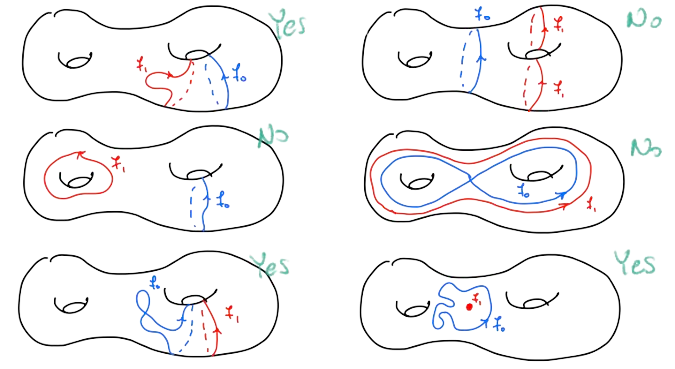
\includegraphics[scale=0.3]{diagrams/homotopies.png} \quad 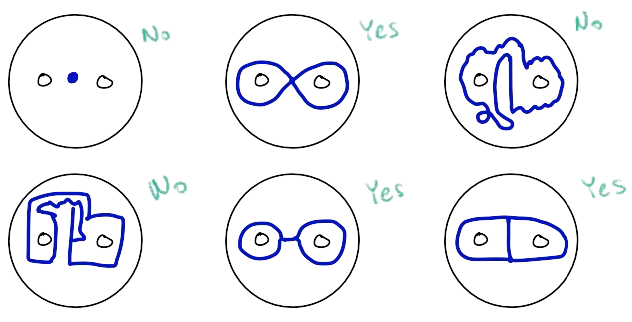
\includegraphics[scale=0.3]{diagrams/defret.png}
    \end{center}
    
\end{exmbox}


\begin{whitebox}
    \textbf{Remark.} 
    \begin{enumerate}
        \item If $\beta$ is a reparameterization of $\alpha$ then $\alpha \simeq \beta$ rel $\set{0,1}$.
        \item $X \cong Y \implies X\simeq Y$ but not converse, e.g. M\"obius band $\simeq S^1 \simeq$ Band $S^1\times I$.
        \item \textit{Fact:} $X\simeq Y$ $\Longleftrightarrow$ $\exists Z$ that deformation retracts to both $X$ and $Y$.
    \end{enumerate}
    
\end{whitebox}

\section{CW Complexes}

\begin{defbox}
    A \emph{CW complex / cell complex} is a space $X$ built as such:
    \begin{enumerate}
        \item Start with a discrete set $X^0$, whose points are \emph{0-cells}.
        \item Let $D^n_{\alpha}$ be $n$-balls (with $\partial D^n_{\alpha} = S^{n-1}_\alpha$). Inductively, form the \emph{$\pmb{n}$-skeleton} $X^n $ as the quotient space of $X^{n-1}\sqcup_\alpha D^n_\alpha$ by identifying $x\sim \phi_\alpha(x)$ where $\phi_\alpha: \partial D^n_\alpha \> X^{n-1}$ are the \emph{attaching maps}. This makes $X^n = X^{n-1} \sqcup_\alpha \text{int}\pr{D^n_\alpha}$ as a set. The $e_\alpha^n=\text{int}\pr{D^n_\alpha}$ are called \emph{$\pmb{n}$-cells}.
        \item One can stop after finite $n$, setting $X=X^n$. Or one can set $X=\bigcup_{n=0}^\infty X^n$, giving it the \textit{weak topology}: $U\subseteq X$ is open $\Leftrightarrow U\cap X^n$ is open in $X^n$ for all $n$.  
    \end{enumerate}
    The \emph{characteristic map} of a cell $e^n_\alpha$ is the map\vspace{-0.5cm}\\
    \begin{align*}
        \Phi_\alpha: D^n_\alpha \hookrightarrow X^{n-1} \sqcup_\beta D^n_\beta \xrightarrow[]{\text{quot}} X^n \hookrightarrow X
    \end{align*}
\end{defbox}

\begin{exmbox}[bottomrule=0pt]
    \begin{enumerate}
        \item A 1-dim CW complex is a \emph{graph}, whose 0-cells are \emph{nodes} and 1-cells are \emph{edges}.\vspace{-0.5cm}
        \begin{center}
            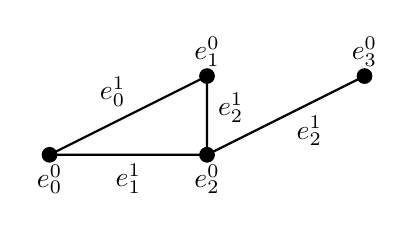
\begin{tikzpicture}
                \draw[thick] (2,0) -- (0,0) -- (2,1) -- (2,0) -- (4,1);
                \fill (0,0) node[below] {$e^0_0$} circle (0.1);
                \fill (2,0) node[below] {$e^0_2$} circle (0.1);
                \fill (2,1) node[above] {$e^0_1$} circle (0.1);
                \fill (4,1) node[above] {$e^0_3$} circle (0.1);
                \draw (0.8,0.8) node {$e^1_0$};
                \draw (1,-0.3) node {$e^1_1$};
                \draw (2.3,0.6) node {$e^1_2$};
                \draw (3.3,0.3) node {$e^1_2$};
            \end{tikzpicture}\vspace{-0.5cm}\\
        \end{center}
        \item $X=T^2$ is a CW complex, with $X^0 = \set{e^0_0}$, $X_1 = X^0 \sqcup e^0_a \sqcup e^0_b$ where $\phi_a \equiv \phi_b \equiv e^0_0$ being constant, and $X^2 = X^1 \sqcup e^2$ with attaching map $\phi:S^1 \> X^1$ given by\vspace{-0.5cm}
        \begin{center}
            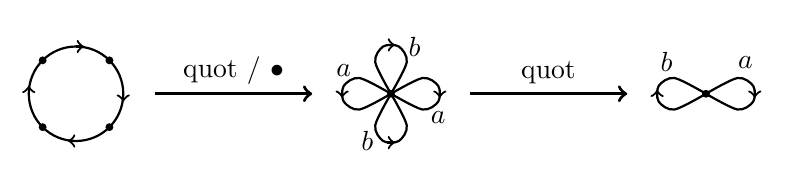
\begin{tikzpicture}
                \draw[thick] (0,0) circle (0.6);
                \draw[thick,->] (0,0.6) -- (0.1,0.6);
                \draw[thick,->] (0,-0.6) -- (-0.1,-0.6);
                \draw[thick,->] (0.6,0) -- (0.6,-0.1);
                \draw[thick,->] (-0.6,0) -- (-0.6,0.1);
                \fill (0.424, 0.424) circle (0.05);
                \fill (-0.424, 0.424) circle (0.05);
                \fill (-0.424, -0.424) circle (0.05);
                \fill (0.424, -0.424) circle (0.05);
                \draw[->, very thick] (1,0) -- (3,0);
                \draw (2,0) node[above] {quot / $\bullet$};
                \draw[thick] plot [smooth] coordinates {(4,0) (3.8, 0.4) (3.9,0.6) (4.1, 0.6) (4.2, 0.4) (4, 0)};
                \draw[thick] plot [smooth] coordinates {(4,0) (3.8, -0.4) (3.9,-0.6) (4.1, -0.6) (4.2, -0.4) (4, 0)};
                \draw[thick] plot [smooth] coordinates {(4,0) (4.4, 0.2) (4.6,0.1) (4.6, -0.1) (4.4, -0.2) (4, 0)};
                \draw[thick] plot [smooth] coordinates {(4,0) (3.6, 0.2) (3.4,0.1) (3.4, -0.1) (3.6, -0.2) (4, 0)};
                \fill (4,0) circle (0.05);
                \draw[thick,->] (3.95,0.62) -- (4.05,0.62);
                \draw[thick,->] (3.95,-0.62) -- (4.05,-0.62);
                \draw[thick,->] (4.62,0.05) -- (4.62,-0.05);
                \draw[thick,->] (3.38,0.05) -- (3.38,-0.05);
                \draw (4.3, 0.6) node {$b$};
                \draw (3.7, -0.6) node {$b$};
                \draw (4.6, -0.3) node {$a$};
                \draw (3.4, 0.3) node {$a$};
                \draw[->, very thick] (5,0) -- (7,0);
                \draw (6,0) node[above] {quot};
                \draw[thick] plot [smooth] coordinates {(8,0) (8.4, 0.2) (8.6,0.1) (8.6, -0.1) (8.4, -0.2) (8, 0)};
                \draw[thick] plot [smooth] coordinates {(8,0) (7.6, 0.2) (7.4,0.1) (7.4, -0.1) (7.6, -0.2) (8, 0)};
                \draw[thick,->] (8.62,0.05) -- (8.62,-0.05);
                \draw[thick,->] (7.38,-0.05) -- (7.38,0.05);
                \draw (7.5, 0.4) node {$b$};
                \draw (8.5, 0.4) node {$a$};
                \fill (8,0) circle (0.05);
            \end{tikzpicture}\vspace{-0.5cm}\\
        \end{center}\textit{Note}: If we swap the direction of two adjacent leaves in the middle step, we get a \emph{Klein bottle}. Attaching maps matter!
        \end{enumerate}
    \end{exmbox}
    \begin{redbox}[toprule=0pt]
    \begin{enumerate}
        \item[3.] The $n$-sphere $S^n$ is a cell complex with two cells $e^0$ and $e^n$, with the attaching map $S^{n-1}\> e^0$. Or, we can inductively attach two $n$-cells to the equator $S^{n-1}$.
        \item[4.] $\R \mathbb{P}^n \cong S^n/(v\sim -v)\cong D^n/(v\sim -v: v\in \partial D^n)$ is a cell complex by attaching an $n$-cell to $\R \mathbb{P}^{n-1}$ via the map $S^{n-1} \twoheadrightarrow \R \mathbb{P}^{n-1}$. We can also have $\R \mathbb{P}^\infty = \bigcup_n \R \mathbb{P}^n$.
    \end{enumerate}
\end{redbox}

\begin{defbox}
    A \emph{subcomplex} of a CW complex $X$ is a closed subspace $A\subseteq X$ that is a union of cells of $X$. The pair $(X,A)$ is a \emph{CW pair}.
\end{defbox}
\begin{exmbox}
    \begin{enumerate}
        \item $\R \mathbb{P}^{k}\subseteq \R \mathbb{P}^n$ is a subcomplex $(k\leq n)$.
        \item $S^k\subseteq S^n$ is not a subcomplex with the two-cell structure, but is a subcomplex using the recursive CW structure.
    \end{enumerate}
\end{exmbox}

\begin{thmbox}
    \begin{itemize}
        \item If $X,Y$ are cell complexes, then $X\times Y$ is a cell complex, whose cells are $e^m_\alpha \times e^n_\beta$ where $e^m_\alpha,e^n_\beta$ are cells of $X,Y$ respectively.
        \item If $(X,A)$ is a CW pair, then the quotient space $X/A$ is a cell complex, whose cells are the cells of $X\setminus A$, and one new 0-cell: the image of $A$ in $X/A$.
    \end{itemize}
    
\end{thmbox}

\begin{defbox}
    $A\subseteq X$ has the \emph{homotopy extension property} if given any map $f_0:X\>Y$ and a homotopy $f_t\mid_A : A\> Y$ of $f_0\mid_A$, we can extend $f_t\mid_A$ to a homotopy $f_t$ on $X$. Equivalently, given any maps $H_1:X\times\set{0}\>Y $ and $H_2:A\times I\> Y$ that agree on $A\times\set{0}$, there exists a map $H:X\times I\>Y$ such that $H$ agrees with both $H_1,H_2$ where their domains meet.
\end{defbox}

\begin{thmbox}
    $A\subseteq X$ has the homotopy extension property if and only if 
    \begin{align*}
        X\times \set{0} \cup A\times [0,1] \text{ is a retract of }X\times[0,1].
    \end{align*}
\end{thmbox}
\textit{Proof.} Let $Z = X\times \set{0} \cup A\times [0,1]$. 
\begin{itemize}
    \item If $A\subseteq X$ has h.e.p then given the maps $H_1: X\times\set{0}\> Z$ and $H_2: A\times I \> Z$ with $$H_1(x,0) = (x,0) \qquad \text{and} \qquad H_2(a,t) = (a,t)$$ we can get an extension $H: X\times I\> Z$ constant on $Z$. Hence $H$ is the retraction.
    \item The converse is easy if we assume $A$ is closed. Say $r:X\times I \> Z$ is a retraction. Given any $H_1,H_2$ as in the definition, we can combine them via the Pasting Lemma to get $H_3: Z \> Y$. Then $H_3 \circ r : X\times I \> Y$ is the required homotopy. For the full proof where $A$ is not necessarily closed, see appendix of [Hatcher].\QED
\end{itemize}

\begin{thmbox}
    If $(X,A)$ is a CW pair, $A$ has the homotopy extension property.
\end{thmbox}
\textit{Proof.} To prove $X\times\set{0} \cup A\times I$ is a retract of $X\times I$, we first prove
\begin{whitebox}
    \textbf{Lemma.} $D^n\times \set{0} \cup \partial D^n \times I$ is a deformation retract of $D^n \times I$.\vspace{0.4cm}\\
    \textit{Proof.} Consider radial projection $r$ from $(\textbf{0},2)\in D^n \times\R$:
    \begin{center}
        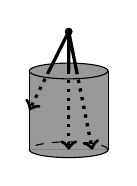
\begin{tikzpicture}
            
            \draw[fill=black, fill opacity=0.4] (0.5,0) arc(0:-180:0.5 and 0.1);
            \draw[dashed] (0.5,0) arc(0:180:0.5 and 0.1);
            \fill[opacity=0.4] (-0.5,0) rectangle (0.5,1);
            \draw[fill=white] (0,1) ellipse (0.5 and 0.1);
            \fill[opacity=0.4] (0,1) ellipse (0.5 and 0.1);
            \draw (-0.5,0) -- (-0.5,1);
            \draw (0.5,0) -- (0.5,1);

            \fill (0,1.5) circle (0.05);

            \draw[->, very thick, dotted] (0,1) -- (0,0);

            \draw[very thick] (0.1,1) -- (0,1.5) -- (0,1);

            \draw[->, very thick, dotted] (0.1,1) -- (0.3,0);

            \draw[very thick] (0,1.5) -- (-0.25, 1);

            \draw[->, very thick, dotted] (-0.25,1) -- (-0.5,0.5);
        \end{tikzpicture}
    \end{center}
    Then $f_t = t \cdot r + (1-t) \cdot \textbf{1}$ is a deformation retract.\qed
\end{whitebox}
Applying the deformation retraction to every $D^n$ attached to $X^{n-1}$ that is not in $A^n$, we get a deformation retraction $H_n$ from $X^n\times I$ onto $X^n\times \set{0}\cup \pr{X^{n-1}\cup A^n}\times I$. Note that concatenating adjacent $H_n$ and $H_{n+1}$ gives a deformation retraction
\begin{align*}
    X^{n+1}\times I &\xrightarrow{H_{n+1}} X^{n+1}\times \set{0}\cup \pr{X^{n}\cup A^{n+1}}\times I\\
    &\xrightarrow{H_n} X^{n+1}\times \set{0}\cup \pr{\pr{X^{n}\times \set{0}\cup \pr{X^{n-1}\cup A^n}\times I}\cup \pr{A^{n+1}\times I}}\\
    &= X^{n+1}\times \set{0} \cup \pr{X^{n-1}\cup A^{n+1}}\times I
\end{align*}
and thus by concatenating all $H_0,H_1,\cdots$ into $[1/4,1/2], [1/8,1/4],\cdots$ we get a deformation retract from $X\times I $ onto $ X\times\set{0} \cup A \times I$. (In the infinite case, there is no continuity problem at $t=0$ since $X$ is given the weak topology).\QED


\begin{thmbox}
    If $(X,A)$ is a CW pair and $A$ is contractible, then the quotient map $X\twoheadrightarrow X/A$ is a homotopy equivalence.
\end{thmbox}
\textit{Proof.} Let $f_t:X\>X$ be a homotopy extension of the contraction of $A$ with $f_0 = \textbf{1}_X$. Since $f_t(A) \subseteq A$ and $f_1(A) = $ pt, we can construct well-defined maps $\ol{f_t}, g$ satisfying
\begin{center}
    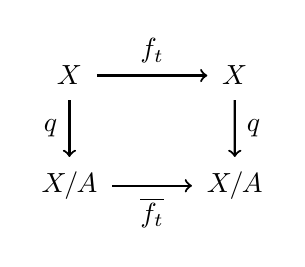
\begin{tikzpicture}[->, thick,main/.style={inner sep = 5pt, minimum size = 0.6cm},edge/.style={midway, inner sep=4pt, minimum size=0.4cm} , scale = 0.7]
    
    \node[main] (00) at (0,0) {$X/A$};
    \node[main] (10) at (3,0) {$X/A$};
    \node[main] (11) at (3,2) {$X$};
    \node[main] (01) at (0,2) {$X$};

    \path
        (01) edge node[edge, above] {$f_t$} (11)
        (11) edge node[edge, right] {$q$} (10)
        (00) edge node[edge, below] {$\ol{f_t}$} (10)
        (01) edge node[edge, left] {$q$} (00)
        ;
    \end{tikzpicture}\qquad
    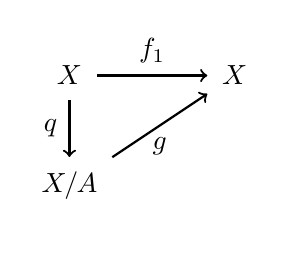
\begin{tikzpicture}[->, thick,main/.style={inner sep = 5pt, minimum size = 0.6cm},edge/.style={midway, inner sep=4pt, minimum size=0.4cm} , scale = 0.7]
    
    \node[main] (00) at (0,0) {$X/A$};
    \node[main] (10) at (3,0) {};
    \node[main] (11) at (3,2) {$X$};
    \node[main] (01) at (0,2) {$X$};

    \path
        (01) edge node[edge, above] {$f_1$} (11)
        (00) edge node[edge, below] {$g$} (11)
        (00) edge[color=white] node[edge, below] {\phantom{$\ol{f_t}$}} (10)
        (01) edge node[edge, left] {$q$} (00)
        ;
    \end{tikzpicture}
\end{center}
Then $g\circ q = f_1 \simeq f_0 = \textbf{1}_X$ and $q(g([x])) = q(g(q(x))= q(f_1(x)) = \ol{f_1}(q(x)) = \ol{f_1}([x])$ and hence $q\circ g = \ol{f_1} \simeq \ol{f_0} = \textbf{1}_{X/A}$, so $g,q$ are homotopy equivalences.

\begin{exmbox}
    \begin{enumerate}
        \item 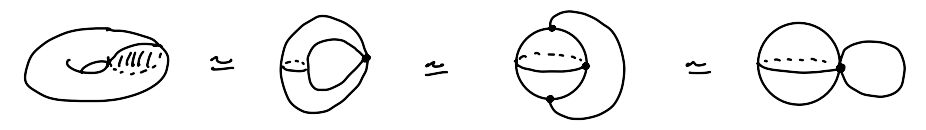
\includegraphics[scale=0.3]{diagrams/homeq1.png}
        \item 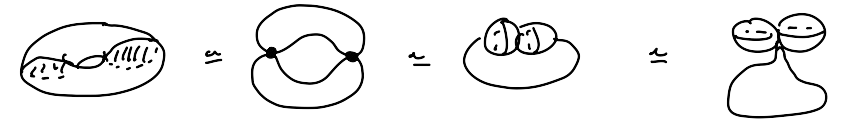
\includegraphics[scale=0.3]{diagrams/homeq2.png}
    \end{enumerate}
\end{exmbox}

\section{Fundamental Groups}\label{FGchap}

\begin{defbox}
    \begin{enumerate}
        \item A \emph{path} on $X$ is $\alpha:I \> X$. Define $\Omega_{x_0}(X) = \set{\text{path }\alpha \mid \alpha(0) = \alpha(1) = x_0}$.
        \item Given paths $\alpha,\beta \in \Omega_{x_0}(X)$, define the \emph{concatenation} $\alpha \cdot \beta\in \Omega_{x_0}(X)$ by
        \begin{align*}
            (\alpha \cdot \beta)(s) = \cases{
            \alpha(2s) & 0\leq s\leq 0.5\\
            \beta(2s-1) & 0.5\leq s \leq 1.
            }
        \end{align*}
        \item Given a path $\gamma \in \Omega_{x_0}(X)$, define the \emph{reversed path} $\ol{\gamma}(t) = \gamma(1-t)$.
        \item The \emph{fundamental group} of $X$ based at $x_0$ is the group
    \begin{align*}
        \pi_1(X,x_0) = \Omega_{x_0}(X)/\sim
    \end{align*}
    where $\alpha \sim \beta \iff \alpha \simeq \beta$ rel $\set{0,1}$, with group law $[\alpha][\beta] = [\alpha \cdot \beta]$ and $[\gamma]^{-1}=\ol{\gamma}$.
    \end{enumerate}
\end{defbox}

\begin{thmbox}
    Let $\gamma$ be a path from $x_0$ to $x_1$. The map $\Phi_\gamma: \pi_1(X,x_1) \> \pi_1(X,x_0)$ by
    $\Phi([\alpha])=[\gamma \cdot \alpha \cdot \ol{\gamma}]$
    is an isomorphism.
\end{thmbox}

\begin{whitebox}
    \textbf{Corollary.} If $X$ is path-connected, $\pi_1(X,x)$ are isomorphic over all $x\in X$ (say $\pi_1(X)$).
\end{whitebox}
\begin{thmbox}
    If $X,Y$ are path-connected, $\pi_1(X\times Y) = \pi_1(X) \times \pi_1(Y)$.
\end{thmbox}
\begin{defbox}
    $X$ is \emph{simply connected} if $X$ is path-connected and $\pi_1(X)$ is trivial.
\end{defbox}

\begin{defbox}\begin{enumerate}
    \item Write $f:(X,x_0)\> (Y,y_0)$ if $f:X\>Y$ and $f(x_0)=y_0$.
    \item The \emph{homomorphism induced} by $f:(X,x_0)\> (Y,y_0)$ is the homomorphism
    \begin{align*}
        f_*: \pi_1(X,x_0) \> \pi_1(X,y_0)
    \end{align*}
    given by $f_*([\alpha]) = [f\circ \alpha]$.
\end{enumerate}
    
\end{defbox}

\begin{thmbox}
    \begin{enumerate}
        \item $(f\circ g)_* = f_* \circ g_*$.
        \item If $f,g:X\>Y$ are homotopic rel $x_0$, then $f_* = g_*$.
        \item If $f:X\> Y$ is a homotopy equivalence, then $f_*$ is an isomorphism.
    \end{enumerate}
\end{thmbox}


\begin{thmbox}\label{FGcircle}
    $\pi_1(S^1) = \Z$.
\end{thmbox}
\textit{Proof.} Let $p: \R\> S^1$ given by $p(\lambda) = \pr{\cos(2\pi\lambda), \sin(2\pi \lambda)}$. The following two facts will be proven in the Covering Spaces chapter.
\begin{whitebox}
    \begin{enumerate}
        \item Given any path $\gamma$ of $S^1$, there exists a unique path $\Tilde{\gamma}$ of $\R$ such that $\Tilde{\gamma}(0)=0$ and $\gamma = p \circ \Tilde{\gamma}$.
        \item Given any homotopy $f_t:I \> S^1$, there exists a unique homotopy $\Tilde{f_t}: I \> \R$ such that $f_t = p \circ \Tilde{f_t}$
    \end{enumerate}
\end{whitebox}
The map $\Phi([\gamma]) = \Tilde{\gamma}(1)\in \Z$ is then a well-defined isomorphism.\QED

\begin{thmbox}
    If $A$ is a retract of $X$, then the inclusion $i:A\xhookrightarrow{} X$ induces an injective homomorphism $i_*$. If $A$ is a defo retract of $X$, then $i_*$ is an isomorphism.
\end{thmbox}
\textit{Proof.} Let $r:X\twoheadrightarrow A$ be a retraction. Then $r\circ i = \textbf{1}\implies r_*\circ i_* = \textbf{1}\implies i_*$ injective. If there is a deformation retraction, then $i$ is a homotopy equivalence and hence $i_*$ is an isomorphism.\QED

\begin{thmbox}
    \textbf{(Brouwer's Fixed Point Theorem)}\\
    $f:D^2\>D^2 \implies f(x) = x$ for some $x\in D^2$.
\end{thmbox}
\textit{Proof.} Otherwise, the map $r$ defined by
\begin{center}
    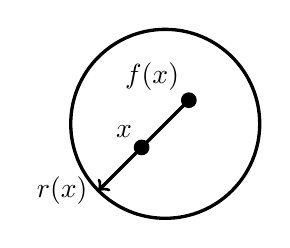
\begin{tikzpicture}
        \draw[very thick] (0,0) circle (1.2);
        \fill (0.3,0.3) node[above left] {$f(x)$} circle (0.1);
        \fill (-0.3,-0.3) node[above left] {$x$} circle (0.1);
        \draw[->, very thick] (0.3,0.3) -- (-0.849,-0.849) node[left] {$r(x)$};
    \end{tikzpicture}
\end{center}
is a retract from $D^2$ to $S^1$, so $i: S^1 \> D^2$ induces an injective $i_*: \Z \> \set{0}$, contradiction.\QED


\begin{thmbox}
    \textbf{(Fundamental Theorem of Algebra)}\\
    Every complex polynomial of positive degree has a root.
\end{thmbox}
\textit{Proof.} Let $f(x) = x^n + a_{n-1}x^{n-1}+\cdots+a_0$ where $n>0$. Assume $f$ has no roots. Then
\begin{align*}
    F(s,t,r) = \pr{re^{2\pi i s}}^n + a_{n-1}\pr{re^{2\pi i s}}^{n-1}t+\cdots+a_0t^n \neq 0 \quad \forall s,t,r.
\end{align*}
Then the homotopy
\begin{align*}
    \frac{F(s,0,1)}{\abs{F(s,0,1)}} \stackrel{t}{\simeq} \frac{F(s,1,1)}{\abs{F(s,1,1)}}  \stackrel{r}{\simeq} \frac{F(s,1,0)}{\abs{F(s,1,0)}} 
\end{align*}
brings the path $e^{2\pi i s n}$, that loops around the circle $n$ times, to the trivial path $1$. This is a contradiction since they correspond to different elements in $\pi_1(S^1)$.\QED

\section{Van Kampen's Theorem} \label{vankampenchap}

\begin{defbox}
    Let $i_1: H \xhookrightarrow{} G_1$ and $i_2: H\xhookrightarrow{} G_2$ be homomorphisms. The \emph{amalgamated free product} of $G_1$ and $G_2$ along $H$, denoted as $G=G_1 *_H G_2$, is the unique group (up to isomorphism) that satisfies
    \begin{enumerate}
        \item[(1)] There exists homomorphisms $\phi_i: G_i\> G$ with $\phi_1 \circ i_1 = \phi_2 \circ i_2$.
        \item[(2)] For any other homomorphisms $\psi_i: G_i\> K$ with $\psi_1 \circ i_1 = \psi_2 \circ i_2$, there exists a unique homomorphism $\psi:G\> K$ with $\psi \circ \phi_i = \psi_i$.
    \end{enumerate}\vspace{-0.7cm}
    \begin{center}
        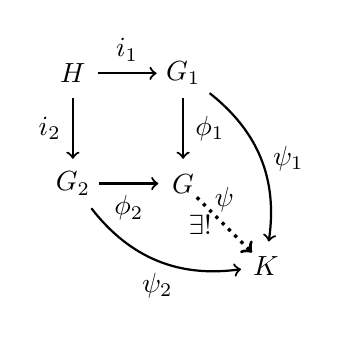
\begin{tikzpicture}[->, thick,main/.style={inner sep = 3pt, minimum size = 0.6cm},edge/.style={midway, inner sep=4pt, minimum size=0.4cm} , scale = 0.7]
    
    \node[main] (00) at (0,0) {$G_2$};
    \node[main] (10) at (2,0) {$G$};
    \node[main] (11) at (2,2) {$G_1$};
    \node[main] (01) at (0,2) {$H$};
    \node[main] (dr) at (3.5,-1.5) {$K$};

    \path
        (01) edge node[edge, above] {$i_1$} (11)
        (11) edge node[edge, right] {$\phi_1$} (10)
        (00) edge node[edge, below] {$\phi_2$} (10)
        (01) edge node[edge, left] {$i_2$} (00)
        (00) edge[bend right=30] node[edge,below] {$\psi_2$} (dr)
        (11) edge[bend left=30] node[edge,right] {$\psi_1$} (dr)
        (2.25,-0.25) edge[dotted, very thick] node[edge,above] {$\psi$} node[edge,left] {$\exists !$} (3.25,-1.25)
        ;
    \end{tikzpicture}
    \end{center}\vspace{-0.5cm}
    If $H=\set{0}$, then $G_1 * G_2 = G_1 *_H G_2$ is just the \emph{free product} of $G_1$ and $G_2$.
\end{defbox}

\begin{whitebox}
    \textbf{Remark.} \begin{enumerate}
        \item Such a group always exists, e.g. if $G_i=\ar{S_i \mid R_i}$ then
    \begin{align*}
        G_1 *_H G_2 = \ar{S_1 \sqcup S_2 \mid R_1 \cup R_2 \cup \set{i_1(h)i_2(h^{-1}): h\in H}}.
    \end{align*}
    Uniqueness follows from the uniqueness of $\psi$ between two such possible groups.
        \item Think of $G_1 *_H G_2$ by first treating $H$ as a common subgroup of $G_1,G_2$, then construct all possible words of finite length with letters from $G_1\cup G_2$. When two adjacent letters in a word both come from the same $G_i$, or if they both belong to $H$, we can further simplify the word.
    \end{enumerate}
\end{whitebox}

\begin{exmbox}
    \begin{enumerate}
        \item The free group with $n$ letters is simply $F_n = \underbrace{\Z * \cdots * \Z}_n$.
        \item The free product of $\Z_2 = \set{1,a,a^2=1}$ and itself $\Z_2 =\set{1,b,b^2=1}$ is
        \begin{align*}
            \Z_2 * \Z_2 = \set{1, a, b, ab, ba, aba, bab, \cdots}
        \end{align*}
        (This is the semi-direct product of $\Z=\ar{c:=ab},\Z_2 = \ar{a}$ with $ac=c^{-1}a$, sometimes called the \textit{infinite dihedral group}.)
        \item If we embed $H=\Z_2$ into the two $\Z_2$'s above by $h\mapsto a$ and $h\mapsto b$, then the free product collapses into
        \begin{align*}
            \Z_2 *_H \Z_2 = \set{1, h, h^2=1
            } = \Z_2
        \end{align*}
    \end{enumerate}
\end{exmbox}

\begin{thmbox}
    \textbf{(Van Kampen's Theorem, two-set version)}\\
    Suppose $X=U\cup V$ where $U,V,U\cap V$ are open and path-connected, then for $x_0\in U\cap V$ we have $\pi_1(X,x_0) = \pi_1(U,x_0) *_{\pi_1(U\cap V, x_0)} \pi_1(V,x_0)$ \quad (with $\pi_1(U\cap V, x_0) \xhookrightarrow{} \pi_1(U, x_0)$ and $\pi_1(U\cap V, x_0) \xhookrightarrow{} \pi_1(V, x_0)$ being the maps induced by the inclusions $U\cap V\xhookrightarrow{} U$ and $U\cap V\xhookrightarrow{} V$ respectively).
\end{thmbox}

\begin{exmbox}
    $\pi_1(S^n) = \set{0}$ for $n\geq 2$ (\textit{high-dim spheres are simply connected}).
    \x $S^n$ is the union of open neighborhoods of the north and south hemisphere, intersecting at the equator $\simeq S^{n-1}$. Hence $\pi_1(S^n) = \pi_1(e^n) *_{\pi_1(S^{n-1})} \pi_1(e^n) = \set{0} *_{\pi_1(S^{n-1})} \set{0} = \set{0}$.
\end{exmbox}

\begin{defbox}
    Suppose $x_0\in X, y_0\in Y$. The \emph{wedge sum} $(X,x_0)\vee (Y,y_0)$ is the space $(X\sqcup Y)/\set{x_0,y_0}$ (gluing $X$ and $Y$ together at $x_0,y_0$). Lazy: $X\vee Y$.
\end{defbox}

\begin{exmbox}
    $S^1\vee S^1$ is the figure-eight, homemorphic to the shape $\infty$.
\end{exmbox}

\begin{thmbox}
    If $\exists$ neighborhoods $x_0\in U, y_0\in V$ in $X,Y$ such that $\set{x_0},\set{y_0}$ are deformation retracts of $U,V$ respectively, then $\pi_1(X\vee Y) = \pi_1(X) \times \pi_1(Y)$.
\end{thmbox}

\textit{Proof.} Let $H_t: U\>U, G_t: V\> V$ be deformation retracts onto $x_0, y_0$ respectively.
\begin{itemize}
    \item We can define $\ol{G_t}: X\vee V \> X \vee V$ by \vspace{-0.7cm}\\
    \begin{center}
        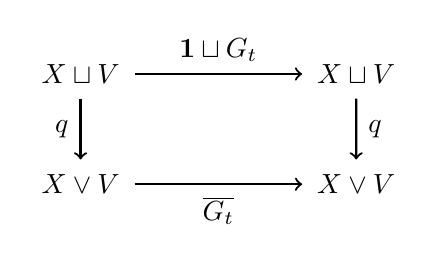
\begin{tikzpicture}[->, thick,main/.style={inner sep = 5pt, minimum size = 0.6cm},edge/.style={midway, inner sep=4pt, minimum size=0.4cm} , scale = 0.7]
        
        \node[main] (00) at (0,0) {$X \vee V$};
        \node[main] (10) at (5,0) {$X \vee V$};
        \node[main] (11) at (5,2) {$X \sqcup V$};
        \node[main] (01) at (0,2) {$X\sqcup V$};
    
        \path
            (01) edge node[edge, above] {$\textbf{1}\sqcup G_t$} (11)
            (11) edge node[edge, right] {$q$} (10)
            (00) edge node[edge, below] {$\ol{G_t}$} (10)
            (01) edge node[edge, left] {$q$} (00)
            ;
        \end{tikzpicture}
    \end{center}\vspace{-0.5cm}
    which is a deformation retraction of $X\vee V$ onto $X\vee \set{y_0} \cong X$. Hence $X\vee V$ deformation retracts onto $X$ and (similarly) $U\vee Y$ deformation retracts onto $Y$.
    \item We claim that $U\vee V\subseteq X\vee Y$ is contractible. The map $F_t: U\vee V \> U \vee V$ defined by\vspace{-0.7cm}\\
    \begin{center}
        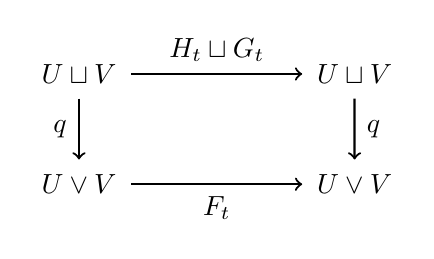
\begin{tikzpicture}[->, thick,main/.style={inner sep = 5pt, minimum size = 0.6cm},edge/.style={midway, inner sep=4pt, minimum size=0.4cm} , scale = 0.7]
        
        \node[main] (00) at (0,0) {$U \vee V$};
        \node[main] (10) at (5,0) {$U \vee V$};
        \node[main] (11) at (5,2) {$U \sqcup V$};
        \node[main] (01) at (0,2) {$U\sqcup V$};
    
        \path
            (01) edge node[edge, above] {$H_t \sqcup G_t$} (11)
            (11) edge node[edge, right] {$q$} (10)
            (00) edge node[edge, below] {$F_t$} (10)
            (01) edge node[edge, left] {$q$} (00)
            ;
        \end{tikzpicture}
    \end{center}\vspace{-0.5cm}
    is a deformation retraction onto $x_0 \in U\vee V$.
    \item By Van Kampen, $\pi_1(X\vee Y) = \pi_1(X\vee V) *_{\pi_1(U\vee V)} \pi_1(U\vee Y)= \pi_1(X) * \pi_1(Y)$.\QED
\end{itemize}
\begin{corollary}
    $\pi_1\pr{\bigvee_{i=1}^n S^1} = F_n$.
\end{corollary}

\begin{thmbox}
    If $\Gamma$ is a connected graph, then $\pi_1(\Gamma) = F_{1-\chi(\Gamma)}$ where $\chi(\Gamma) = \abs{V(\Gamma)} - \abs{E(\Gamma)}$ is the \emph{Euler characteristic} of $\Gamma$.
\end{thmbox}
\textit{Proof.} Let $T$ be a spanning tree of $\Gamma$, which is contractible. Then by collapsing $T$, the graph $\Gamma/T \simeq \Gamma$ is a wedge sum of $\abs{E(\Gamma - T)}$ circles. Hence $\pi_1(\Gamma) = F_n$ where
\begin{align*}
    n = \abs{E(\Gamma)} - \abs{E(T)} = \abs{E(\Gamma)} - \pr{\abs{V(T)}-1} = 1 - \chi(T).\tag*{\QED}
\end{align*}

\begin{thmbox}
    If $i: H\> G = \ar{S\mid R}$, then $G*_H \set{0} = \ar{S \mid R \cup i(H)}$
\end{thmbox}

\begin{exmbox}
    We can compute $\pi_1\pr{T^2}$ as follows:\vspace{-0.2cm}
    \begin{center}
        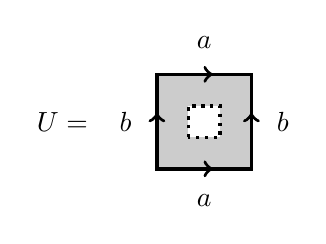
\begin{tikzpicture}
            \draw[very thick, fill=black, fill opacity =0.2] (0,0) -- (1.2,0) -- (1.2,1.2) -- (0,1.2) -- cycle;
            \draw[very thick, ->] (0.7,0) -- (0.71,0);
            \draw (0.6,-0.4) node {$a$};
            \draw[very thick, ->] (0.7,1.2) -- (0.71,1.2);
            \draw (0.6,1.6) node {$a$};
            \draw[very thick, ->] (1.2, 0.7) -- (1.2, 0.71);
            \draw (1.6,0.6) node {$b$};
            \draw[very thick, ->] (0, 0.7) -- (0, 0.71);
            \draw (-0.4,0.6) node {$b$};
            \draw[very thick, dotted, fill=white] (0.4,0.4) rectangle (0.8,0.8);
            \draw (-1.2,0.6) node {$U=$};
        \end{tikzpicture}
        \qquad
        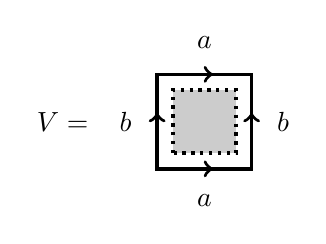
\begin{tikzpicture}
            \draw[very thick] (0,0) -- (1.2,0) -- (1.2,1.2) -- (0,1.2) -- cycle;
            \draw[very thick, ->] (0.7,0) -- (0.71,0);
            \draw (0.6,-0.4) node {$a$};
            \draw[very thick, ->] (0.7,1.2) -- (0.71,1.2);
            \draw (0.6,1.6) node {$a$};
            \draw[very thick, ->] (1.2, 0.7) -- (1.2, 0.71);
            \draw (1.6,0.6) node {$b$};
            \draw[very thick, ->] (0, 0.7) -- (0, 0.71);
            \draw (-0.4,0.6) node {$b$};
            \draw[very thick, dotted, fill=black, fill opacity =0.2] (0.2,0.2) rectangle (1,1);
            \draw (-1.2,0.6) node {$V=$};
        \end{tikzpicture}
        \qquad
        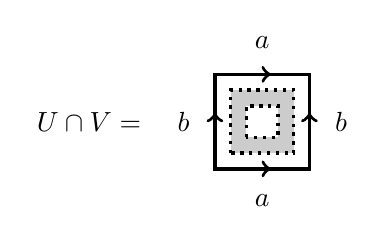
\begin{tikzpicture}
            \draw[very thick] (0,0) -- (1.2,0) -- (1.2,1.2) -- (0,1.2) -- cycle;
            \draw[very thick, ->] (0.7,0) -- (0.71,0);
            \draw (0.6,-0.4) node {$a$};
            \draw[very thick, ->] (0.7,1.2) -- (0.71,1.2);
            \draw (0.6,1.6) node {$a$};
            \draw[very thick, ->] (1.2, 0.7) -- (1.2, 0.71);
            \draw (1.6,0.6) node {$b$};
            \draw[very thick, ->] (0, 0.7) -- (0, 0.71);
            \draw (-0.4,0.6) node {$b$};
            \draw[very thick, dotted, fill=black, fill opacity =0.2] (0.2,0.2) rectangle (1,1);
            \draw[very thick, dotted, fill=white] (0.4,0.4) rectangle (0.8,0.8);
            \draw (-1.6,0.6) node {$U\cap V=$};
        \end{tikzpicture}
    \end{center}
    \vspace{-0.7cm}
    \begin{align*}
        \pi_1(T^2) = \pi_1(U) *_{\pi_1(U\cap V)} \pi_1(V) = \ar{a,b} *_{\Z} \set{0} = \ar{a,b \mid aba^{-1}b^{-1}} = \Z^2.
    \end{align*}
\end{exmbox}

\chapterpart{Fundamental Group of CW Complexes}

\begin{thmbox}\label{cwcpxthm}
\begin{enumerate}
    \item Let $X^2$ be a CW complex obtained from $X^1$ by attaching 2-cells $e^2_\alpha$ via $\phi_\alpha: \partial D^2_\alpha \> X^1$. For each $\alpha$, let $\gamma_\alpha$ be a path on $X^1$ from $x_0$ to a point $z_\alpha\in \partial D^2_\alpha$.
    \begin{align*}
        \pi_1(X^2, x_0) = \pi_1 (X^1,x_0)/N
    \end{align*}
    where $N$ is the normal closure of the subgroup of $\pi_1(X^1, x_0)$ generated by paths $\br{\gamma_\alpha\cdot \phi_\alpha\cdot\ol{\gamma_\alpha}}$ (treating $\phi_\alpha$ as a closed path based at $z_\alpha$).
    \item Attaching $n$-cells $(n\geq 3)$ does not change the fundamental group, i.e. $$\pi_1(X, x_0) = \pi_1(X^2,x_0)$$
\end{enumerate}
    
\end{thmbox}

\begin{exmbox}
    \begin{enumerate}
        \item For the Klein bottle $K$, we have $\pi_1(K) = \ar{a,b}/N$ where $N$\\is generated by $aba^{-1}b$, so $\pi_1(K) = \ar{a,b \mid aba^{-1}b}$.
        \vspace{-2.2cm}\begin{center}
            \hfill 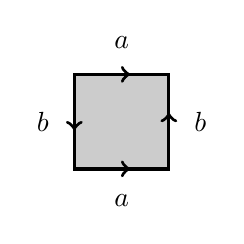
\begin{tikzpicture}
            \draw[very thick, fill=black, fill opacity =0.2] (0,0) -- (1.2,0) -- (1.2,1.2) -- (0,1.2) -- cycle;
            \draw[very thick, ->] (0.7,0) -- (0.71,0);
            \draw (0.6,-0.4) node {$a$};
            \draw[very thick, ->] (0.7,1.2) -- (0.71,1.2);
            \draw (0.6,1.6) node {$a$};
            \draw[very thick, ->] (1.2, 0.7) -- (1.2, 0.71);
            \draw (1.6,0.6) node {$b$};
            \draw[very thick, ->] (0, 0.5) -- (0, 0.49);
            \draw (-0.4,0.6) node {$b$};
        \end{tikzpicture}
        \end{center}\vspace{-1cm}
        \item If $X$ is obtained by attaching a single 2-cell to a circle $\C^\times$ via $\phi(z)=z^n$, then $\pi_1(X)=\ar{x \mid x^n} = \Z_n$. In particular, $\pi_1(\R \mathbb{P}^2) = \Z_2$.
    \end{enumerate}
\end{exmbox}
\begin{corollary}
    Given any group $G$, there exists a space $X$ with $\pi_1(X)=G$.
\end{corollary}
\textit{Proof.} Write $G=\ar{S\mid R}$ and attach 2-cells (according to $R$) to the wedge sum $\bigvee_{s\in S} S^1_s$.\QED
\newpage
\textit{Proof of Theorem \ref{vankampenchap}.\ref{cwcpxthm}.} First expand $X^2$ by bulging up the $e^2_\alpha$'s and then adding strips $S_\alpha = I\times I$ along each $\gamma_\alpha$. Pick a $y_\alpha \in e^2_\alpha$ that is not on the strip. Call this larger space $Z$.
\begin{center}
    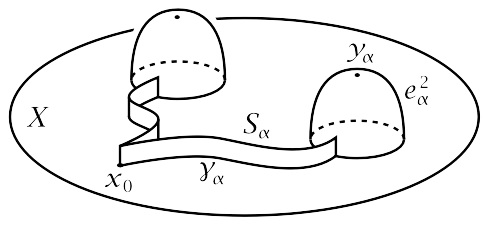
\includegraphics[scale=0.4]{diagrams/cwcpxFG.png}
\end{center}
We then slice this space along half the height of the $S_\alpha$'s, and consider an open neighborhood of the top and bottom parts $U,V$ respectively (e.g. $U=Z\setminus X^1$ and $V=Z\setminus \bigcup_\alpha\set{y_\alpha}$). $U$ is contractible while $V$ deformation retracts to $X^1$. Hence
\begin{align*}
    \pi_1(X^2,x_0) = \pi_1(Z,x_0) = \pi_1(U,x_0) *_{\pi_1(U\cap V, x_0)} \pi_1(V,x_0) = \set{0} *_{\pi_1(U\cap V, x_0)} \pi_1(X^1,x_0).
\end{align*}
So it remains to show that $\pi_1(U\cap V, x_0)$ is generated by the $[\gamma_\alpha \cdot \phi_\alpha \cdot \ol{\gamma_\alpha}]$: We can apply Van Kampen again on $U\cap V$ by covering it with the open sets $A_\alpha = U\cap V \setminus \bigcup_{\beta\neq \alpha} D^2_\beta$ which deformation retract to a circle and hence is generated by $\gamma_\alpha \cdot \phi_\alpha \cdot \ol{\gamma_\alpha}$. This shows (1).
\\ \\
\quad To show (2), we perform the same procedure. However, in the last step, the $A_\alpha$ deformation retract to spheres, which are simply connected. The finite $X^n$ case follows from induction. If $X$ is infinite-dimensional, any closed loop at $x_0$ is compact and hence is contained in some finite $X^n$ anyway.\QED

\begin{defbox}
\begin{enumerate}
    \item Let $\Sigma, \Sigma'$ be surfaces. The \emph{connect sum}, $\Sigma \ \# \ \Sigma'$ is defined by
    \begin{align*}
        \pr{\Sigma \setminus \text{int}\pr{D^2}} \sqcup \pr{\Sigma' \setminus \text{int}\pr{D^2}} / \sim
    \end{align*}
    where $\sim$ identifies boundary points.
    \item The \emph{surface of genus $\pmb{g}$} is $\Sigma_g=\underbrace{T^2 \ \# \ \cdots \ \# \ T^2}_n \ \# \ S^2$ (The $g$-holed torus).
\end{enumerate}
    
\end{defbox}

\begin{exmbox}\vspace{-0.5cm}
    \begin{center}
        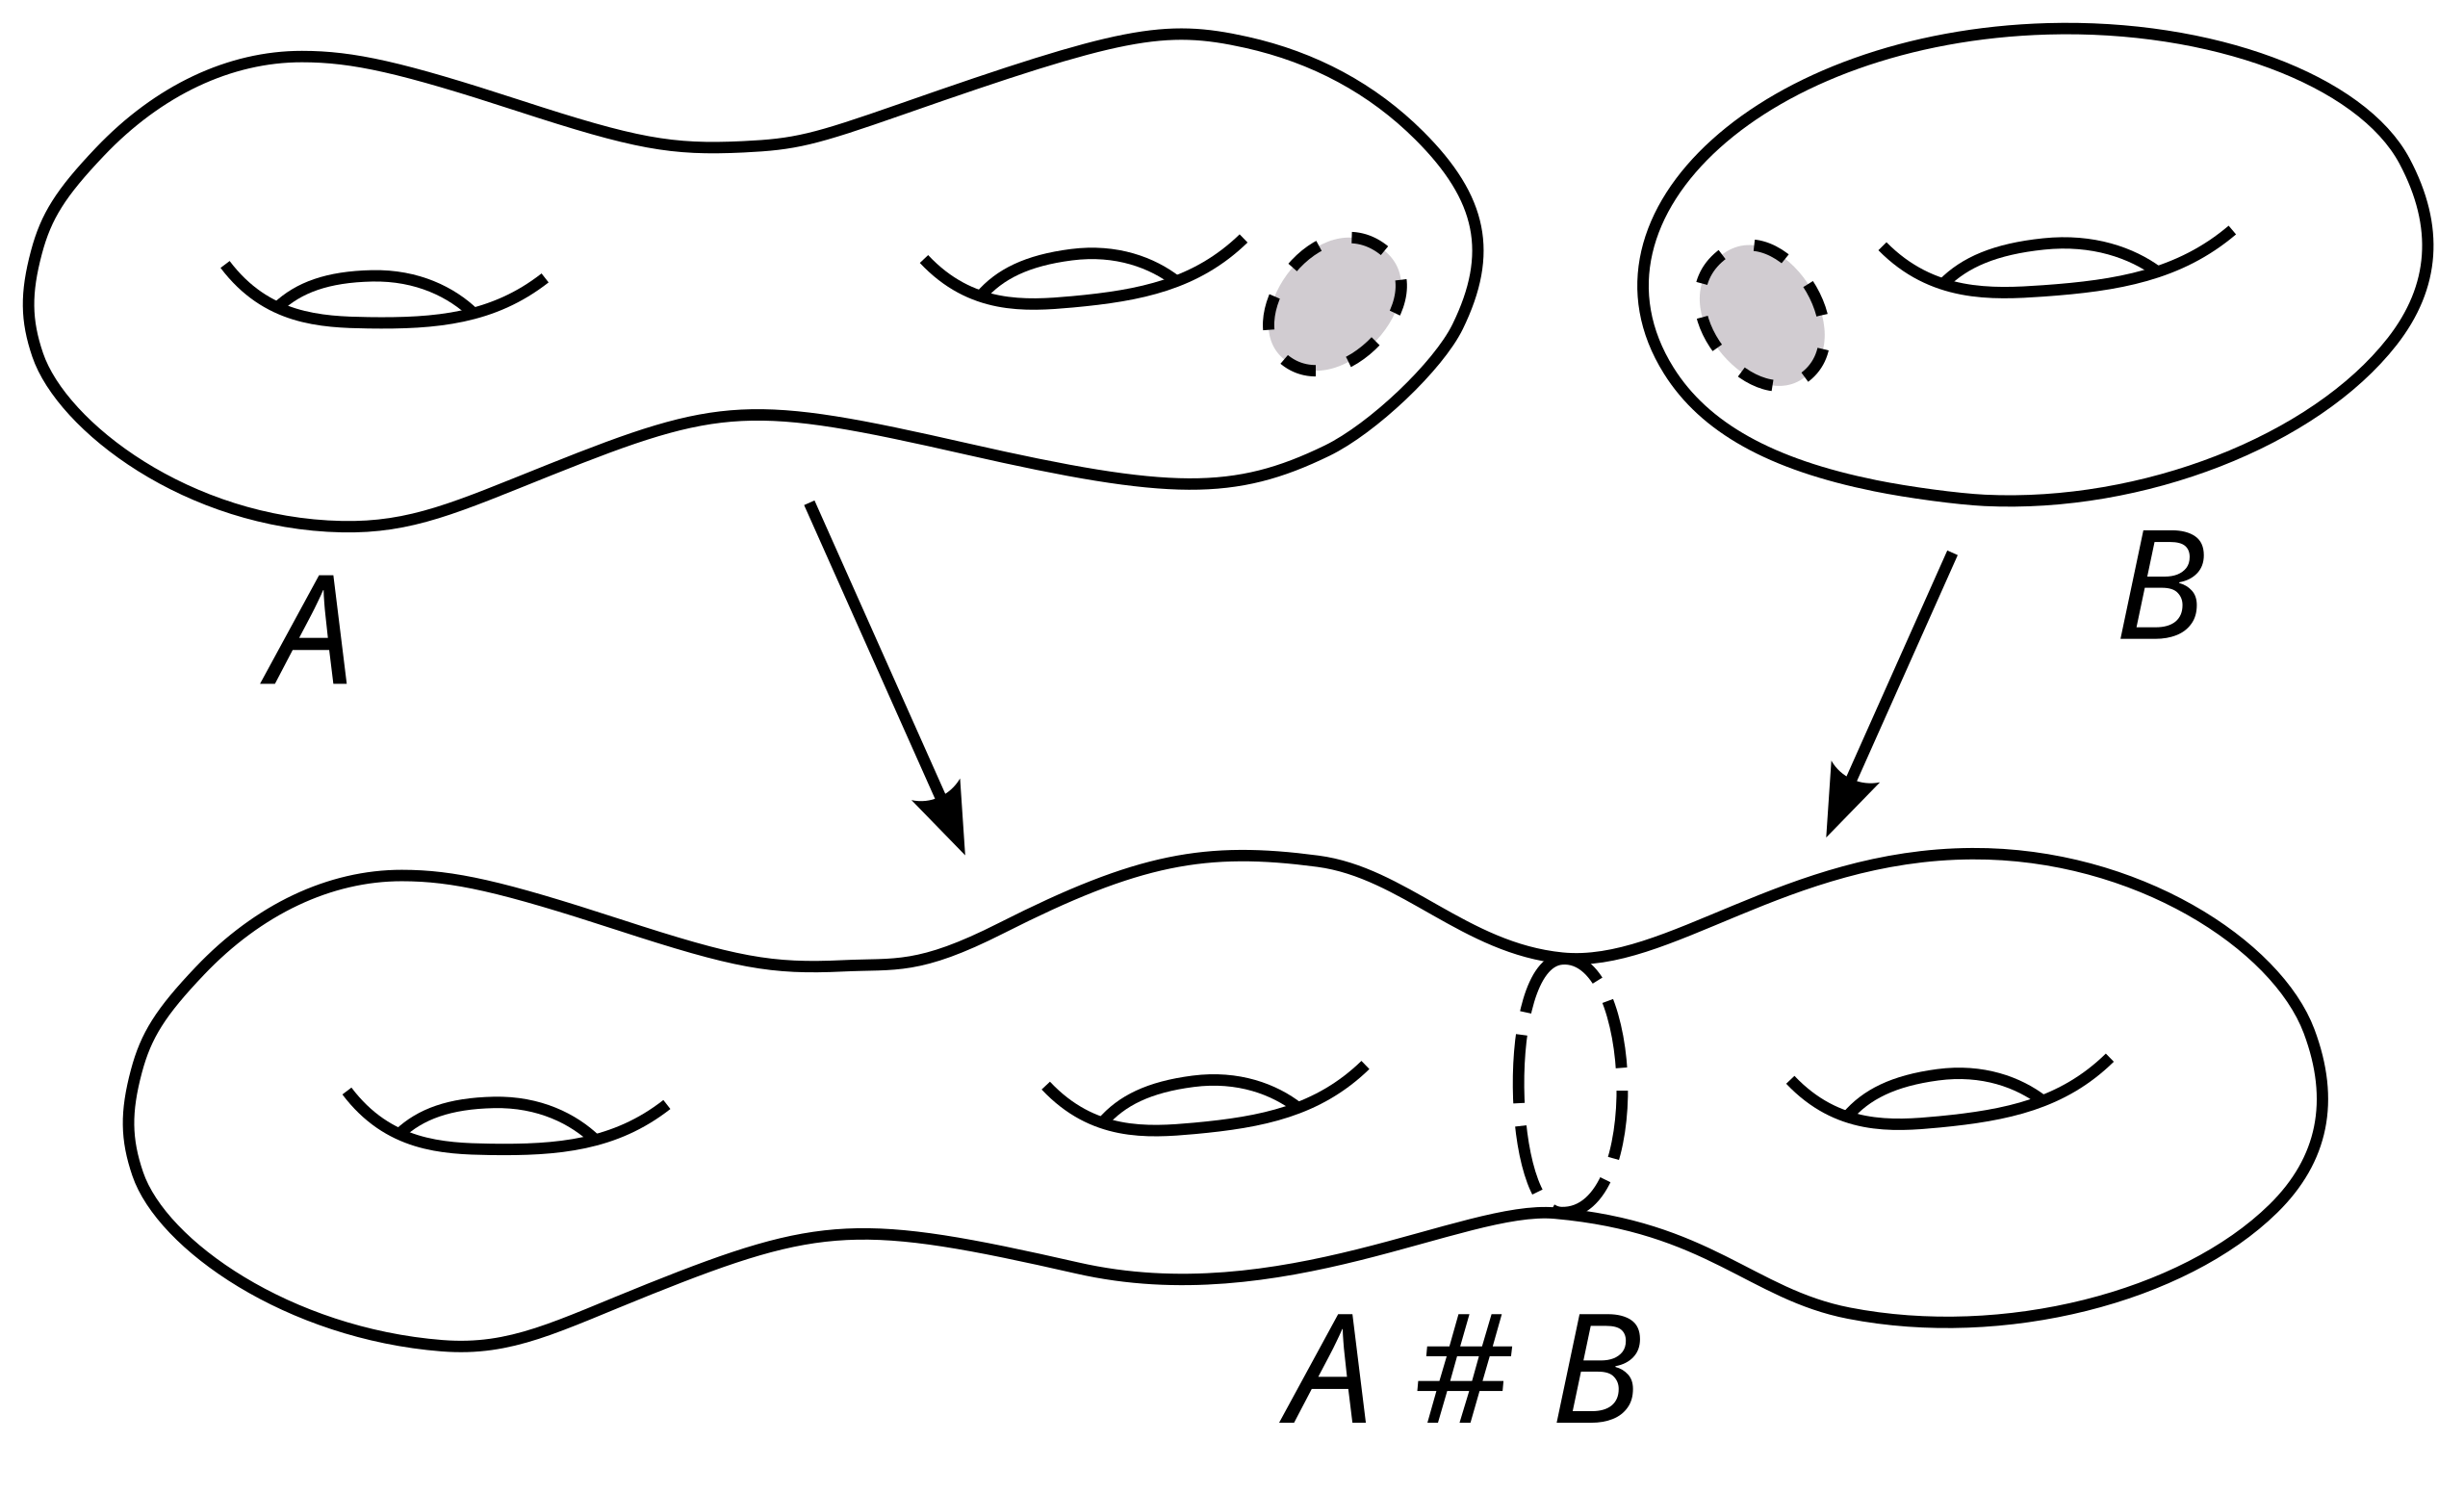
\includegraphics[scale=0.05]{diagrams/Connected_sum.svg.png}
    \end{center}
\end{exmbox}

\begin{thmbox}
    $\pi_1\pr{\Sigma_g} = \ar{a_1,b_1,a_2,b_2,\cdots,a_g,b_g \mid a_1b_1a^{-1}_1b_1^{-1}\cdots a_gb_ga_g^{-1}b_g^{-1}}$
\end{thmbox}
\textit{Diagram.}\vspace{-0.7cm}
\begin{center}
    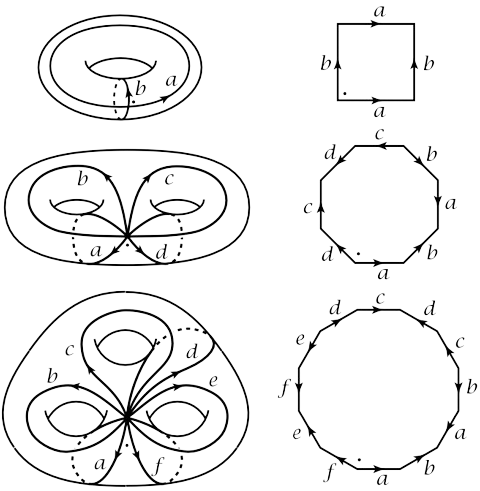
\includegraphics[scale=0.5]{diagrams/genusgsurface.png}
\end{center}

\section{Covering Spaces}

\begin{defbox}
    \begin{enumerate}
        \item A \emph{covering space} of $X$ is a space $\Tilde{X}$ with a map $p:\Tilde{X}\> X$ such that every $x\in X$ admits a neighborhood $U$ such that $f^{-1}(U) = \bigsqcup_\alpha \Tilde{U}_\alpha$ (a disjoint union of open sets) where each $p\mid_{\Tilde{U}_\alpha}$ is a homeomorphism. We say that $U$ is \emph{evenly covered} by the \emph{sheets} $\Tilde{U}_\alpha$.
        \item A \emph{lift} of a map $f:Y\>X$ is a map $\Tilde{f}: Y \> \Tilde{X}$ with $f = p\circ \Tilde{f}$.\vspace{-0.4cm}
        \begin{center}
            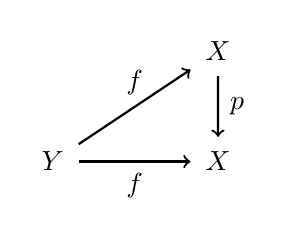
\begin{tikzpicture}[->, thick,main/.style={inner sep = 5pt, minimum size = 0.6cm},edge/.style={midway, inner sep=4pt, minimum size=0.4cm} , scale = 0.7]
    
            \node[main] (00) at (0,0) {$Y$};
            \node[main] (10) at (3,0) {$X$};
            \node[main] (11) at (3,2) {$\Tilde{X}$};
        
            \path
                (11) edge node[edge, right] {$p$} (10)
                (00) edge node[edge, above] {$\Tilde{f}$} (11)
                (00) edge node[edge, below] {$f$} (10)
                ;
            \end{tikzpicture}
        \end{center}
    \end{enumerate}
\end{defbox}
\begin{exmbox}
    \begin{enumerate}
        \item $p:\R\>S^1$, $p(\lambda) = e^{2\pi i\lambda}$.\vspace{-0.5cm}
        \begin{center}
            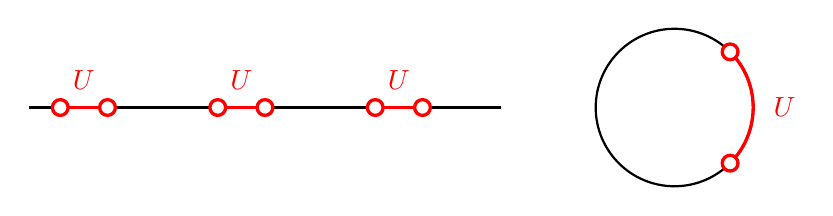
\begin{tikzpicture}
                \draw[thick] (-4.2,0) -- (1.8,0);
                
                \draw[very thick, color=red] (-3.8,0) -- (-3.2,0);
                \draw[very thick, color=red, fill = white] 
                    (-3.8,0) circle (0.1)
                    (-3.2,0) circle (0.1);
                \draw[color=red] (-3.5,0.1) node[above] {$\Tilde{U}$};

                \draw[very thick, color=red] (-1.8,0) -- (-1.2,0);
                \draw[very thick, color=red, fill = white] 
                    (-1.8,0) circle (0.1)
                    (-1.2,0) circle (0.1);
                \draw[color=red] (-1.5,0.1) node[above] {$\Tilde{U}$};

                \draw[very thick, color=red] (0.2,0) -- (0.8,0);
                \draw[very thick, color=red, fill = white] 
                    (0.2,0) circle (0.1)
                    (0.8,0) circle (0.1);
                \draw[color=red] (0.5,0.1) node[above] {$\Tilde{U}$};
                
                \draw[thick] (4,0) circle (1);
                \draw[very thick, color=red] (4.707, 0.707) arc (45:-45:1);
                \draw[very thick, color=red, fill = white] (4.707,0.707) circle (0.1);
                \draw[very thick, color=red, fill = white] (4.707,-0.707) circle (0.1);
                \draw[color=red] (5.4,0) node {$U$};
            \end{tikzpicture}
        \end{center}
        \item $p_n:S^1\>S^1$, $p_n(z) = z^n$.\vspace{-0.3cm}
        \begin{center}
            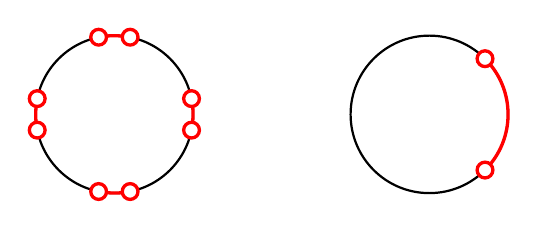
\begin{tikzpicture}

                \draw[thick] (0,0) circle (1);
                \draw[very thick, color=red] (0.98, 0.2) arc (11.25:-11.25:1);
                \draw[very thick, color=red, fill = white] (0.98,0.2) circle (0.1);
                \draw[very thick, color=red, fill = white] (0.98,-0.2) circle (0.1);
                \draw[very thick, color=red] (-0.98, -0.2) arc (191.25:168.75:1);
                \draw[very thick, color=red, fill = white] (-0.98,-0.2) circle (0.1);
                \draw[very thick, color=red, fill = white] (-0.98,0.2) circle (0.1);
                \draw[very thick, color=red] (-0.2, 0.98) arc (101.25:78.75:1);
                \draw[very thick, color=red, fill = white] (-0.2,0.98) circle (0.1);
                \draw[very thick, color=red, fill = white] (0.2,0.98) circle (0.1);
                \draw[very thick, color=red] (0.2, -0.98) arc (281.25:258.75:1);
                \draw[very thick, color=red, fill = white] (0.2,-0.98) circle (0.1);
                \draw[very thick, color=red, fill = white] (-0.2,-0.98) circle (0.1);
                
                \draw[thick] (4,0) circle (1);
                \draw[very thick, color=red] (4.707, 0.707) arc (45:-45:1);
                \draw[very thick, color=red, fill = white] (4.707,0.707) circle (0.1);
                \draw[very thick, color=red, fill = white] (4.707,-0.707) circle (0.1);
            \end{tikzpicture}
        \end{center}
        \item A few covering spaces of $S^1\vee S^1$, as 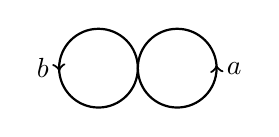
\begin{tikzpicture}
\draw[thick] (3.5, -2) circle (0.5); 
\draw[thick, ->] (3.00069, -2.02617) -- (3.00122, -2.03488);
\draw[thick] (3.0, -2.0) node[left] {$b$};
\draw[thick] (4.5, -2) circle (0.5); 
\draw[thick, ->] (4.99931, -1.97383) -- (4.99878, -1.96512);
\draw[thick] (5.0, -2.0) node[right] {$a$};
\end{tikzpicture}:\vspace{-0.5cm}
        \begin{center}
            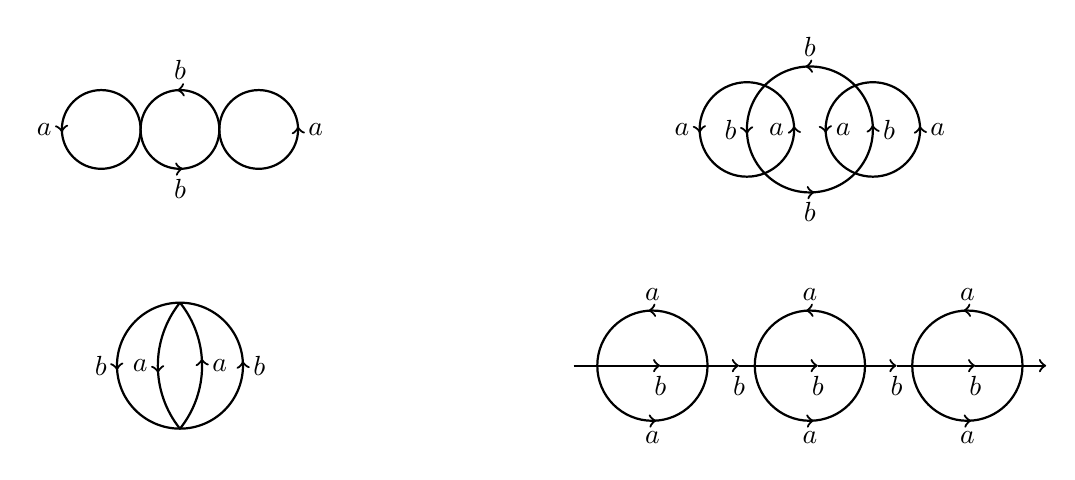
\begin{tikzpicture}
\draw[thick] (0, 0) circle (0.5); 
\draw[thick, ->] (-0.02617, 0.49931) -- (-0.03488, 0.49878);
\draw[thick] (0.0, 0.5) node[above] {$b$};
\draw[thick, ->] (0.02617, -0.49931) -- (0.03488, -0.49878);
\draw[thick] (-0.0, -0.5) node[below] {$b$};
\draw[thick] (-1, 0) circle (0.5); 
\draw[thick, ->] (-1.49931, -0.02617) -- (-1.49878, -0.03488);
\draw[thick] (-1.5, 0.0) node[left] {$a$};
\draw[thick] (1, 0) circle (0.5); 
\draw[thick, ->] (1.49931, 0.02617) -- (1.49878, 0.03488);
\draw[thick] (1.5, 0.0) node[right] {$a$};
\draw[thick] (8, 0) circle (0.8); 
\draw[thick, ->] (8.7989, 0.04187) -- (8.79805, 0.05581);
\draw[thick] (8.8, 0.0) node[right] {$b$};
\draw[thick, ->] (7.95813, 0.7989) -- (7.94419, 0.79805);
\draw[thick] (8.0, 0.8) node[above] {$b$};
\draw[thick, ->] (7.2011, -0.04187) -- (7.20195, -0.05581);
\draw[thick] (7.2, 0.0) node[left] {$b$};
\draw[thick, ->] (8.04187, -0.7989) -- (8.05581, -0.79805);
\draw[thick] (8.0, -0.8) node[below] {$b$};
\draw[thick] (7.2, 0) circle (0.6); 
\draw[thick, ->] (7.79918, 0.0314) -- (7.79854, 0.04185);
\draw[thick] (7.8, 0.0) node[left] {$a$};
\draw[thick, ->] (6.60082, -0.0314) -- (6.60146, -0.04185);
\draw[thick] (6.6, 0.0) node[left] {$a$};
\draw[thick] (8.8, 0) circle (0.6); 
\draw[thick, ->] (9.39918, 0.0314) -- (9.39854, 0.04185);
\draw[thick] (9.4, 0.0) node[right] {$a$};
\draw[thick, ->] (8.20082, -0.0314) -- (8.20146, -0.04185);
\draw[thick] (8.2, 0.0) node[right] {$a$};
\draw[thick] (0, -3) circle (0.8); 
\draw[thick, ->] (0.7989, -2.95813) -- (0.79805, -2.94419);
\draw[thick] (0.8, -3.0) node[right] {$b$};
\draw[thick, ->] (-0.7989, -3.04187) -- (-0.79805, -3.05581);
\draw[thick] (-0.8, -3.0) node[left] {$b$};
\draw[thick] (-0.00029, -2.19977) arc (141.34019:218.65981:1.281); 
\draw[thick, ->] (-0.27924, -3.06704) -- (-0.27788, -3.08936);
\draw[thick] (-0.281, -3.0) node[left] {$a$};
\draw[thick] (0.00029, -3.80023) arc (-38.65981:38.65981:1.281); 
\draw[thick, ->] (0.27924, -2.93296) -- (0.27788, -2.91064);
\draw[thick] (0.281, -3.0) node[right] {$a$};
\draw[thick] (8, -3) circle (0.7); 
\draw[thick, ->] (7.96336, -2.30096) -- (7.95117, -2.30171);
\draw[thick] (8.0, -2.3) node[above] {$a$};
\draw[thick, ->] (8.03664, -3.69904) -- (8.04883, -3.69829);
\draw[thick] (8.0, -3.7) node[below] {$a$};
\draw[thick] (6, -3) circle (0.7); 
\draw[thick, ->] (5.96336, -2.30096) -- (5.95117, -2.30171);
\draw[thick] (6.0, -2.3) node[above] {$a$};
\draw[thick, ->] (6.03664, -3.69904) -- (6.04883, -3.69829);
\draw[thick] (6.0, -3.7) node[below] {$a$};
\draw[thick] (10, -3) circle (0.7); 
\draw[thick, ->] (9.96336, -2.30096) -- (9.95117, -2.30171);
\draw[thick] (10.0, -2.3) node[above] {$a$};
\draw[thick, ->] (10.03664, -3.69904) -- (10.04883, -3.69829);
\draw[thick] (10.0, -3.7) node[below] {$a$};
\draw[thick,->] (5,-3) -- (6.1,-3) node[below] {$b$};
\draw[thick,->] (6.1,-3) -- (7.1,-3) node[below] {$b$};
\draw[thick,->] (7.1,-3) -- (8.1,-3) node[below] {$b$};
\draw[thick,->] (8.1,-3) -- (9.1,-3) node[below] {$b$};
\draw[thick,->] (9.1,-3) -- (10.1,-3) node[below] {$b$};
\draw[thick,->] (10.1,-3) -- (11,-3);
\end{tikzpicture}
        \end{center}
    \end{enumerate}
\end{exmbox}

\begin{thmbox}
    Let $Y$ be a connected space and $f:Y\>X$. If two lifts $\Tilde{f}_1,\Tilde{f}_2:Y\>\Tilde{X}$ agree at some point $y\in Y$, then $\Tilde{f}_1=\Tilde{f}_2$.
\end{thmbox}
\textit{Proof.} For any $z\in Y$, there is a neighborhood $U$ of $f(z)$ that is evenly covered by sheets $\Tilde{U}_\alpha$. 
\begin{itemize}
    \item $\set{z\in Y: \Tilde{f}_1(z) = \Tilde{f}_2(z)}$ is open: Suppose $\Tilde{f}_1(z) = \Tilde{f}_2(z)\in \Tilde{U}_\beta$, then by continuity there exists a neighborhood $z\in V$ with $\Tilde{f}_1(V) ,\Tilde{f}_2(V)\subseteq \Tilde{U}_\beta$. Then
    \begin{align*}
        \Tilde{f}_1|_V = p\mid_{\Tilde{U}_\beta}^{-1}\circ\  p\mid_{\Tilde{U}_\beta} \circ\  \Tilde{f}_1\mid _V = p\mid_{\Tilde{U}_\beta}^{-1} \circ\  f\mid _V = \Tilde{f}_2|_V.
    \end{align*}\vspace{-0.7cm}
    \item $\set{z\in Y: \Tilde{f}_1(z) = \Tilde{f}_2(z)}$ is closed: $\Tilde{f}_1(z) \neq \Tilde{f}_2(z) \implies \Tilde{f}_1(z)\in \Tilde{U}_{\beta_1}, \Tilde{f}_2(z)\in \Tilde{U}_{\beta_2} \ (\beta_1\neq\beta_2)$. By continuity there exists a neighborhood $z\in V$ with $\Tilde{f}_i(V)\subseteq \Tilde{U}_{\beta_i}$.
\end{itemize}
Since $Y$ is connected, $Y=\set{z\in Y: \Tilde{f}_1(z) = \Tilde{f}_2(z)}$.\QED

\begin{thmbox}
    \textbf{(Homotopy Lifting Property)}\\
    Given a homotopy $f_t:Y \> X$ and a lift $\Tilde{f}_0: Y \> \Tilde{X}$ of $f_0$, there exists a unique homotopy $\Tilde{f}_t: Y\>\Tilde{X}$ of $f_t$ that agrees with $\Tilde{f}_0$.
\end{thmbox}
\begin{whitebox}
    \textbf{Remark.} The two facts used in Theorem \ref{FGchap}.\ref{FGcircle} follow from the case $Y=$ pt and $Y=I$.
\end{whitebox}
\textit{Proof.} Use the $H(x,t) = f_t(x)$ notation.
\begin{whitebox}
    \textbf{Lemma.} For any $y\in Y$, there exists open $y\in V$ and $0=t_0 < t_1 <\cdots< t_n=1$ such that each $H\pr{V\times [t_i,t_{i+1}]}$ is contained in some evenly covered $U_i$.\vspace{0.3cm}\\
    \textit{Proof.} Fix $y$. For each $t\in I$ there exists a neighborhood $U_t$ of $H(y,t)$ that is evenly covered, and there exists a basis $V_t\times W_t \subseteq Y\times I$ with $(y,t)\in V_t\times W_t \subseteq H^{-1}\pr{U_t}$. Since the $W_t$ cover $I$ which is compact, we have a finite subcover $W_{s_0},\cdots,W_{s_m}$ of $I$ and hence we can take $V = V_{s_0}\cap \cdots \cap V_{s_m}$ and $t_i$ the endpoints of all $W_{s_k}$.
\end{whitebox}
We first prove the theorem by fixing $y$ and restricting $f_t$ on a neighborhood $V\subseteq Y$. By induction, suppose $\Tilde{H}$ has been constructed over $V\times[0,t_i]$. Let $U\supseteq H(V\times [t_i,t_{i+1}])$ be evenly covered by sheets $\Tilde{U}_\alpha$. Let $\Tilde{H}(y,t_i)\in \Tilde{U}_\beta$, then by the pasting lemma we can construct $\Tilde{H}\mid_{V'\times [0,t_{i+1}]}$ by composing $H$ with $p\mid_{U_\beta}^{-1}$, after restricting $V$ to $V'$ by intersecting the pre-image of $\Tilde{U}_\beta$. Relabelling $V'$ as $V$, after a finite number of steps, we constructed $\Tilde{f}_t$ on a neighborhood $V$ of $y$. Note that such $\Tilde{f}_t$ is unique at each $y\in V$ since $\set{y}\times I$ is connected.
\x
To construct $\Tilde{f}_t$ on the entire $Y$, we construct a unique $\Tilde{f}$ on a neighborhood $V_y$ at every $y\in Y$. By uniqueness on each $\set{y}\times I$, the $\Tilde{f}$'s agree on the overlaps, so it is well-defined. By the same uniqueness, the entire $\Tilde{f}$ is unique.\QED

\begin{thmbox}
Let $p_*: \pi_1\pr{\Tilde{X},\Tilde{x}_0}\> \pi_1(X,x_0)$ be induced by $p$.
    \begin{enumerate}
        \item $p_*$ is injective.
        \item $\text{Im}(p_*) = \set{[\alpha]\in\pi_1(X,x_0): \Tilde{\alpha}(0) = \Tilde{\alpha}(1) = \Tilde{x}_0}$.
    \end{enumerate}
\end{thmbox}
\textit{Proof.} Suppose $p_*\pr{[\beta]}=0$. Then $p\circ \beta\simeq$ constant rel $\set{0,1}$. This nullhomotopy has a unique lift in $\Tilde{X}$, which gives a nullhomotopy for $\beta$, i.e. $[\beta]=0$. This proves (1).
\x
For (2), we have $p_*([\beta]) = [p\circ \beta] = \br{\Tilde{\beta}}$.\QED

\begin{thmbox}
    If $X,\Tilde{X}$ are path-connected, then $\abs{p^{-1}(x_0)} = \br{\pi_1(X,x_0): \text{Im}(p_*)}$ (There is a bijection between each preimage of $x_0$ and each coset of $\text{Im}(p_*)$).
\end{thmbox}

\begin{defbox}
A space $Y$ is \emph{locally} \textbf{[insert property]} if for all $y\in Y$ and any neighborhood $y\in U$, there exists a neighborhood $y\in V\subseteq U$ that has the property.
    
\end{defbox}
\begin{thmbox}
    Say $f:(Y,y_0)\>(X,x_0)$ where $Y$ is path-conn and locally path-conn. $$\exists \Tilde{f}:(Y,y_0)\> \pr{\Tilde{X},\Tilde{x}_0}\  \Longleftrightarrow \ \text{Im}\pr{f_*} \subseteq \text{Im}\pr{p_*}$$
\end{thmbox}
\textit{Proof.} For $(\Rightarrow)$, $f=p\circ \Tilde{f}\implies f_* = p_* \circ \Tilde{f}_*$. For $(\Leftarrow)$, suppose $\text{Im}\pr{f_*} \subseteq \text{Im}\pr{p_*}$. Pick for each $y\in Y$ a path $\gamma_y$ from $y_0$ to $y$, then define $\Tilde{f}(y) = \widetilde{f\circ \gamma_y}(1)$ where  $\widetilde{f\circ \gamma_y}(0) = \Tilde{x}_0$.
\begin{itemize}
    \item $\Tilde{f}$ is well-defined: Let $\gamma_1,\gamma_2$ be two paths from $y_0$ to $y$. Then $\br{\gamma_1 \cdot \ol{\gamma_2}} \in \pi_1(Y,y_0)$ and hence exists $[\alpha]\in \pi_1\pr{\Tilde{X},\Tilde{x}_0}$ with $p\circ \alpha \simeq f \circ \gamma_1 \cdot \ol{\gamma_2}$ rel $\set{0,1}$. This homotopy $H_t$ has a unique lift $\Tilde{H}_t$ with $\Tilde{H}_0 = \alpha$. Since $H_1 = (f\circ \gamma_1) \cdot (f\circ \gamma_2)$, by uniqueness we have $\Tilde{H}_1 = \widetilde{f\circ \gamma_1} \cdot \widetilde{f\circ \gamma_2}$, and thus $\widetilde{f\circ \gamma_1}(1) = \Tilde{H}_1 (0.5)  = \widetilde{f\circ \gamma_2}(1)$.
    \item $\Tilde{f}$ is a lift: $p\circ \Tilde{f}(y) = p \circ 
    \widetilde{f\circ \gamma_y} (1) = f\circ \gamma_y(1) = f(y)$.
    \item $\Tilde{f}$ is continuous: Let $W$ be a neighborhood of $\Tilde{f}(y)$. Let $f(y)\in U$ be evenly covered by $\Tilde{U}_\alpha$, and $\Tilde{f}(y) \in \Tilde{U}$. Since $f$ is continuous, $\exists $ neighborhood $y\in V'$ with $f(V') \subseteq p\pr{\Tilde{U}\cap W}$. By local path-connectedness, let $y\in V\subseteq V'$ be a path-connected neighborhood. Then any path from $y_0$ to $y$ can be extended to a path from $y_0$ to any $z\in V$. This eventually shows $\Tilde{f}(V) \subseteq \Tilde{U} \cap W$.\QED
\end{itemize}

\begin{defbox}
    \begin{enumerate}
        \item A space $X$ is \emph{semilocally simply connected} if for all $x\in X$ there exists a neighborhood $x\in U$ where $\pi_1(U,x)\> \pi_1(X,x)$ is trivial.
        \item $X$ is \emph{`nice'} if it is path-conn, locally path-conn and semilocally simply conn.
        \item $p:\Tilde{X}\> X$ is a \emph{universal cover} of $X$ if $X$ is path-conn and $\Tilde{X}$ is simply conn.
        \item Two covering spaces $p_i:\Tilde{X}_i\> X$ are \emph{isomorphic} if there exists a homeomorphism $\phi:\Tilde{X}_1\>\Tilde{X}_2 $ with $p_2 \circ \phi = p_1$.
    \end{enumerate}
\end{defbox}

\begin{thmbox}
    CW complexes are locally contractible and locally path-connected.
\end{thmbox}

\begin{exmbox}
    The \textit{Hawaiian Earring} $H$ consisting of the union of all circles in $\R^2$ with center $(1/n,0)$ and radius $1/n$ for each $n\in\N^*$ is not semilocally simply connected because any neighborhood of $(0,0)$ contains a full circle, which contains loops that cannot be nullhomotopic in $H$.
    \begin{center}
        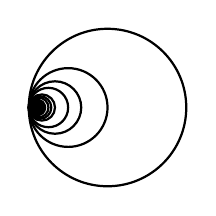
\begin{tikzpicture}
            \draw[thick] (1,0) circle (1);
            \draw[thick] (0.5,0) circle (0.5);
            \draw[thick] (0.333,0) circle (0.333);
            \draw[thick] (0.25,0) circle (0.25);
            \draw[thick] (0.1666,0) circle (0.1666);
            \draw[thick] (0.143,0) circle (0.143);
            \draw[thick] (0.125,0) circle (0.125);
            \fill (0.111,0) circle (0.111);
        \end{tikzpicture}\qquad
        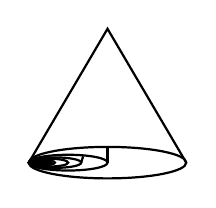
\begin{tikzpicture}
            \draw[thick] (1,0) circle (1 and 0.2);
            \draw[thick] (0.5,0) circle (0.5 and 0.1);
            \draw[thick] (0.333,0) circle (0.333 and 0.0666);
            \draw[thick] (0.25,0) circle (0.25 and 0.05);
            \draw[thick] (0.1666,0) circle (0.1666 and 0.0333);
            \draw[thick] (0.143,0) circle (0.143 and 0.0286);
            \draw[thick] (0.125,0) circle (0.125 and 0.025);
            \fill (0.111,0) circle (0.111 and 0.0222);
            \draw[thick] (0,0) -- (1,1.7) -- (2,0);
            \draw[thick] (1,0) -- (1,0.2);
            \draw[thick] (0.666,0) -- (0.69,0.08);
        \end{tikzpicture}\ \
        \qquad
        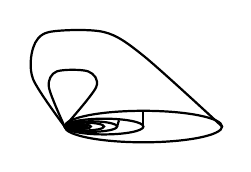
\begin{tikzpicture}
            \draw[thick] (1,0) circle (1 and 0.2);
            \draw[thick] (0.5,0) circle (0.5 and 0.1);
            \draw[thick] (0.333,0) circle (0.333 and 0.0666);
            \draw[thick] (0.25,0) circle (0.25 and 0.05);
            \draw[thick] (0.1666,0) circle (0.1666 and 0.0333);
            \draw[thick] (0.143,0) circle (0.143 and 0.0286);
            \draw[thick] (0.125,0) circle (0.125 and 0.025);
            \fill (0.111,0) circle (0.111 and 0.0222);
            \draw[thick] plot [smooth] coordinates {(0,0) (0.4,0.5) (0.3,0.7) (-0.1, 0.7) (-0.2,0.5) (0,0)};
            \draw[thick] plot [smooth] coordinates {(2,0) (1,0.9) (0.5,1.2) (-0.2, 1.2) (-0.4,1) (-0.4,0.6) (0,0)};
            \draw[thick] (1,0) -- (1,0.2);
            \draw[thick] (0.666,0) -- (0.69,0.08);
        \end{tikzpicture}
    \end{center}
    However, if we consider the \textit{cone} obtained from $H$, defined by $CH = (H\times I)/(H\times\set{0})$, which is simply connected since it is contractible, then $CH$ is semilocally simply connected. If we join the tip of the cone to the limit point at the base, then we form a space that is not simply connected (it is homotopy equivalent to $S^1$) but still semilocally simply connected.
\end{exmbox}

\begin{thmbox}
    \begin{enumerate}
        \item If $X$ is nice, then $X$ has a universal cover.
        \item If $X$ is nice, for any subgroup $H\subseteq \pi_1(X,x_0)$ there exists a covering space $p_H: \Tilde{X}_H\> X$ such that $\text{Im}\pr{p_{H*}} = H$.
    \end{enumerate}
\end{thmbox}
\textit{Proof of (1).} We use a Lemma and 5 steps.
\begin{whitebox}
    \textbf{Lemma.} $\scr{B} = \set{U\subseteq X: U\text{ open, path-conn, $\pi_1(U)\>\pi_1(X)$ trivial}}$ is a basis for the topology of a nice $X$.\vspace{0.3cm}\\
    \textit{Proof.} $\scr{B}$ covers $X$ since $X$ is nice. Suppose $x\in U\cap V$ where $U,V\in \scr{B}$. Since $X$ is locally path-conn, there exists path-connected $x\in W\subseteq U\cap V$, which means $\pi_1(W,x)\> \pi_1(U,x) \xrightarrow{\text{triv}} \pi_1(X,x) \implies W\in \scr{B}$. Hence $\scr{B}$ is a basis. To prove the second part, given any open $x\in W$, choose open $x\in V$ via semilocal simply connectedness, then pick a open and path-connected $U\subseteq V\cap W$ via local path-connectedness. Then $U\in \scr{B}$ with $U\subseteq W$. \QED
\end{whitebox}
\begin{enumerate}
    \item Define $\Tilde{X} = \set{[\gamma]\mid \gamma : I\> X, \gamma(0) = x_0}$ with $[\gamma ]=[\delta] \iff \gamma \simeq \delta$ rel $\set{0,1}$. Define the covering map $p:\Tilde{X}\> X$ by $p([\gamma]) = \gamma(1)$. 
    \item Define the topology on $\Tilde{X}$ as follows: Given $U\in \scr{B}$ and $[\gamma]\in \Tilde{X}$ with $\gamma(1)\in U$, define
    \begin{align*}
        U_{[\gamma]} = \set{[\gamma \cdot \eta]\mid \eta: I\> U \text{ with }\eta(0) =\gamma(1)}
    \end{align*}
    Then $\set{U_{[\gamma]}}_{[\gamma]}$ is a basis (Exercise; ($*$) Note that $[\delta]\in U_{[\gamma]}\implies U_{[\delta]}=U_{[\gamma]}$), and we generate the topology from it.
    \item Claim: $p:U_{[\gamma]}\> U$ is a homeomorphism.
    \begin{itemize}
        \item Surjective: $U$ path-conn $\implies \forall x\in U, \exists \text{path $\eta$ from $\gamma(1)$ to $x$} \implies p([\gamma\cdot \eta]) =x$.
        \item Injective: $p([\gamma\cdot \eta]) = p([\gamma\cdot \eta']) \implies \eta(1) = \eta'(1)$. Since $\pi_1(U)\>\pi_1(X) $ is trivial, $\eta \simeq \eta'\implies [\gamma\cdot \eta]=[\gamma\cdot \eta']$.
        \item Homeo: Note that $\set{B\cap U}_{B\in\scr{B}}$ and $\set{B_{[\delta]}\cap U_{[\gamma]}}_{B\in \scr{B}}$ are bases for $U$ and $U_{[\gamma]}$ respectively, and (1) $p\pr{B_{[\delta]}\cap U_{[\gamma]}} = B\cap U$; and (2) $p^{-1}\pr{B\cap U}\cap U_{[\gamma]} = B_{[\delta]}\cap U_{[\gamma]}$ for any $[\delta]\in U_{[\gamma]}$ with $\delta(1)\in B$ since $B_{[\delta]}\subseteq U_{[\delta]} \stackrel{(*)}{=} U_{[\gamma]}$ and $p\mid_{V_{[\delta]}}$ is bijective.
    \end{itemize}
    \item $p$ is a covering map: Given any $U\in \scr{B}$, $p^{-1}(U) = \bigcup_{[\gamma]} U_{[\gamma]}$ which is a disjoint union of equivalence classes due to $(*)$.
    \item $\Tilde{X}$ is simply connected: Let $[x_0]=$ class of constant paths. Given any $[\gamma]\in \Tilde{X}$, the path $\gamma_t(s) = \gamma(\min(s,t))$ form $\gamma(0)$ to $\gamma(t)$ brings $[x_0]$ to $[\gamma]$, and thus $\Tilde{X}$ is path-connected. To show $\pi_1\pr{\Tilde{X}, [x_0]} = 0$, we show $\text{Im}(p_*) = \set{0}$:
    \begin{align*}
        [\alpha]\in \text{Im}(p_*) \implies [x_0] = \Tilde{\alpha}(0) = \Tilde{\alpha}(1) = [\alpha] \implies [\alpha] = 0.\tag*{\QED}
    \end{align*}
\end{enumerate}
\textit{Proof of (2).} Consider the equivalence relation $\sim$ on the universal cover $\Tilde{X}$ defined by
\begin{align*}
    [\gamma] \sim [\delta] \iff \gamma(1)=\delta(1)\text{ and } [\gamma\cdot \ol{\delta}] \in H.
\end{align*}
Then $X_H = \Tilde{X}/\sim$ is a covering space of $X$. To show $\text{Im}\pr{p_{H*}} = H$: For any $[\alpha]\in\pi_1(X,x_0)$, we have a lift $\Tilde{\alpha}=\alpha_t$ from $[\Tilde{x_0}]$ to $[\alpha]$, so
\begin{align*}
    [\alpha] \in H \iff [\Tilde{x}_0] \sim [\alpha] \iff \Tilde{\alpha}(0) =\Tilde{\alpha}(1) \iff [\alpha] \in \text{Im}(p_{H*})
\end{align*}

\begin{thmbox}
    Let $\Tilde{X}$ be path-connected. Then $p_*\pr{\pi_1\pr{\Tilde{X},\Tilde{x}_0}}$ is conjugate to $p_*\pr{\pi_1\pr{\Tilde{X},\Tilde{x}_1}}$ for any $\Tilde{x}_0,\Tilde{x}_1 \in p^{-1}(x_0)$.
\end{thmbox}
\textit{Proof.} Conjugate using any path  from $\Tilde{x}_0$ to $\Tilde{x}_1$.\QED


\begin{thmbox}
    \textbf{(Classification Theorem of Covering Spaces)}\\
    If $X$ is nice, there is a bijective \emph{Galois correspondence} between
    \begin{align*}
        \begin{Bmatrix}
            \text{conj. classes of}\\
            \text{subgrps of $\pi_1(X,x_0)$}
        \end{Bmatrix} \ \longleftrightarrow \ \begin{Bmatrix}
            \text{isom. classes of path-}\\
            \text{conn. covers $\Tilde{X}\>X$}
        \end{Bmatrix}
    \end{align*}
\end{thmbox}

\textit{Proof.} We prove that $p_1: \Tilde{X}_1\>X$ and $p_2:\Tilde{X}_2 \> X$ are isomorphic if and only if $\text{Im}(p_{1*})$ and $\text{Im}(p_{2*})$ are conjugate in $\pi_1(X)$.
\begin{itemize}
    \item Assume $p_1\cong p_2$. Then $\text{Im}(p_{1*})= \text{Im}(p_{2*}\circ \phi_*) = p_{2*} \pr{\pi_1\pr{\Tilde{X}_2, \phi\pr{\Tilde{x}_1}}}$ which is conjugate to $p_{2*}\pr{\pi_1\pr{\Tilde{X}_2, \Tilde{x}_2}}$ since $p_2 \circ \phi \pr{\Tilde{x}_1} = p_1\pr{\Tilde{x}_1} = x_0 = p_2\pr{\Tilde{x}_2}$.
    \item Suppose $\text{Im}(p_{1*}) = [\alpha]^{-1} \text{Im}(p_{2*}) [\alpha] $. Let $\Tilde{\alpha}: I\> \Tilde{X}_2$ be a lift of $\alpha$ based at $\Tilde{x}_2$. Then
    \begin{align*}
        p_{2*}\pr{\pi_1\pr{\Tilde{X}_2, \Tilde{\alpha}(1)}} = p_{1*}\pr{\pi_1\pr{\Tilde{X}_1, \Tilde{x}_1}}
    \end{align*}
    so there exists lifts $\Tilde{p}_1: \pr{\Tilde{X}_1,\Tilde{x}_1}\> \pr{\Tilde{X}_2,\Tilde{\alpha}(1)}, \Tilde{p}_1: \pr{\Tilde{X}_2,\Tilde{\alpha}(1)}\> \pr{\Tilde{X}_1,\Tilde{x}_1}$ with
    \begin{center}
        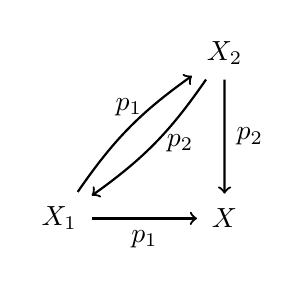
\begin{tikzpicture}[->, thick,main/.style={inner sep = 5pt, minimum size = 0.6cm},edge/.style={midway, inner sep=4pt, minimum size=0.4cm} , scale = 0.7]
    
            \node[main] (00) at (0,0) {$\Tilde{X}_1$};
            \node[main] (10) at (3,0) {$X$};
            \node[main] (11) at (3,3) {$\Tilde{X}_2$};
        
            \path
                (11) edge node[edge, right] {$p_2$} (10)
                (00) edge[bend left=10] node[edge, above] {$\Tilde{p}_1$} (11)
                (11) edge[bend left=10] node[edge, right] {$\Tilde{p}_2$} (00)
                (00) edge node[edge, below] {$p_1$} (10)
                ;
            \end{tikzpicture}
    \end{center}
    Since $\Tilde{p}_2\circ \Tilde{p}_1$ and $\textbf{1}$ agree at $\Tilde{x}_1$ and ar both lifts of $p_1: \Tilde{X}_1 \> X$ to $\Tilde{X}_1$, we have $\Tilde{p}_2\circ \Tilde{p}_1 = \textbf{1}$ and similarly $\Tilde{p}_1\circ \Tilde{p}_2 = \textbf{1}$. Thus $p_1\cong p_2$.\QED
\end{itemize}

\section{Regular Coverings}
\begin{defbox}
    \begin{enumerate}
        \item A \emph{deck transformation} is a self-isomorphism $\Tilde{X}\> \Tilde{X}$ of a covering space $p:\Tilde{X}\> X$. The group of deck transformations is denoted $\text{Aut}(\Tilde{X})$.
        \item A covering space is \emph{regular} if for each $x\in X$ and $\Tilde{x}, \Tilde{x}'\in p^{-1}(x)$, there exists $\phi \in \text{Aut}(\Tilde{X})$ with $\phi(\Tilde{x}) =\Tilde{x}'$.
    \end{enumerate}
    
\end{defbox}

\begin{exmbox}
    $\text{Aut}(\R) = \Z$.
\end{exmbox}

\begin{thmbox}
    $\phi \in \text{Aut}(\Tilde{X})$ is completely determined by $\phi(\Tilde{x}_0)$ when $\Tilde{X}$ is path-connected and locally path-connected.
\end{thmbox}
\textit{Proof.} $\phi$ is a lift to $\Tilde{X}$, which is uniquely determined by where it sends some point.\QED

\begin{thmbox}
    Suppose $X$ is nice. Then $p:\Tilde{X}\> X$ is regular if and only if $\text{Im}(p_*)$ is normal. When this is true, $\text{Aut}(\Tilde{X}) = \pi_1(X,x_0)/\text{Im}(p_*)$.
\end{thmbox}
\textit{Proof.} $p$ is regular $\iff$ for any $\Tilde{x}, \Tilde{x}'\in p^{-1}(x)$ there exists a lift $\phi$ where\begin{center}
        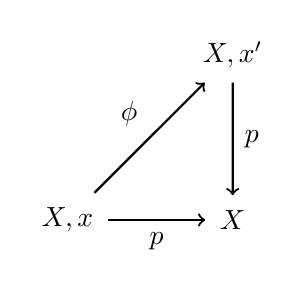
\begin{tikzpicture}[->, thick,main/.style={inner sep = 5pt, minimum size = 0.6cm},edge/.style={midway, inner sep=4pt, minimum size=0.4cm} , scale = 0.7]
    
            \node[main] (00) at (0,0) {$\pr{\Tilde{X},\Tilde{x}}$};
            \node[main] (10) at (3,0) {$X$};
            \node[main] (11) at (3,3) {$\pr{\Tilde{X},\Tilde{x}'}$};
        
            \path
                (11) edge node[edge, right] {$p$} (10)
                (00) edge node[edge, above left] {$\phi$} (11)
                (00) edge node[edge, below] {$p$} (10)
                ;
            \end{tikzpicture}
    \end{center}
    which is equivalent to $p_*\pr{\pi_1\pr{\Tilde{X},\Tilde{x}}}=p_*\pr{\pi_1\pr{\Tilde{X},\Tilde{x}'}}\ \forall \Tilde{x},\Tilde{x}'$, i.e. $p_*\pr{\pi_1\pr{\Tilde{X},\Tilde{x}}}$ is normal. To prove the second part, consider the map $\pi_1(X,x_0)\> \text{Aut}(\Tilde{X})$ is $p_*(\pi_1(X,x_0))$ given by $[\alpha]\mapsto \phi_\alpha$ where $\phi_\alpha(\Tilde{\alpha}(0)=\Tilde{x}_0) = \Tilde{\alpha}(1)$.
    \begin{itemize}
        \item It is a homomorphism: Since a lift of $\alpha \cdot \beta$ is $\Tilde{\alpha}\cdot \phi_\alpha(\Tilde{\beta})$, so 
        \begin{align*}
            [\alpha][\beta] \mapsto \phi_{\alpha\cdot\beta}(\Tilde{x}_0) = \phi_\beta \circ \phi_\alpha(\Tilde{x}_0) \implies \phi_{\alpha\cdot \beta} = \phi_\beta \phi_\alpha.
        \end{align*}
        \item It is injective: $[\alpha]\mapsto 0 \iff [\alpha]\in p_*\pr{\pi_1\pr{\Tilde{X},\Tilde{x}}}$.
        \item It is surjective: Fix a path $\gamma$ in $\Tilde{X}$ from $\Tilde{x}_0$ to $\Tilde{x}_1\in p^{-1}(x_0)$. Then $[p\circ \gamma]\in\pi_1(X,x_0)$ has lift $\gamma$.\QED
    \end{itemize}

    \begin{exmbox} A covering space of $S^1\vee S^1$: 
        \begin{center}
            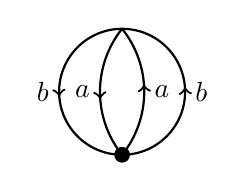
\begin{tikzpicture}
            \draw[thick] (0, -3) circle (0.8); 
            \fill (0,-3.8) circle (0.1);
            \draw[thick, ->] (0.7989, -2.95813) -- (0.79805, -2.94419);
            \draw[thick] (0.8, -3.0) node[right] {$b$};
            \draw[thick, ->] (-0.7989, -3.04187) -- (-0.79805, -3.05581);
            \draw[thick] (-0.8, -3.0) node[left] {$b$};
            \draw[thick] (-0.00029, -2.19977) arc (141.34019:218.65981:1.281); 
            \draw[thick, ->] (-0.27924, -3.06704) -- (-0.27788, -3.08936);
            \draw[thick] (-0.281, -3.0) node[left] {$a$};
            \draw[thick] (0.00029, -3.80023) arc (-38.65981:38.65981:1.281); 
            \draw[thick, ->] (0.27924, -2.93296) -- (0.27788, -2.91064);
            \draw[thick] (0.281, -3.0) node[right] {$a$};
            \end{tikzpicture}
        \end{center}
        $\text{Im}(p_*) = \ar{a^2, ab^{-1},ab}\subseteq \ar{a,b} = \pi_1(S^1\vee S^1,x_0)$ is normal, hence
        \begin{align*}
            \text{Aut}(\Tilde{X}) = \ar{a,b \mid a^2, ab^{-1},ab } = \Z_2.
        \end{align*}
        
    \end{exmbox}
\end{document}
